\documentclass{article} % Loads settings for the document layout

\usepackage[utf8]{inputenc}
\usepackage[T1]{fontenc}
\usepackage{currvita}
\usepackage{graphicx}
\graphicspath{ {images/} }
\title{Mrežno računarstvo - skripta}


% Main document

\begin{document} % The document starts here

\maketitle % Creates the titlepage
\pagenumbering{gobble} % Turns off page numbering
\newpage % Starts a new page
\pagenumbering{arabic} % Turns on page numbering

\section{Komponente mreže, tipovi veza, primeri mreža, mreže prema dimenziji, međumreže}
(preuzeto sa slajdova)
\subsection{Komponente mreže}
Delovi mreže su:\\ 
- \textit{aplikacija}, odnosno korisnik čija je funkcija da koristi mrežu. Primeri za aplikaciju su Skype, iTunes, Amazon.\\
- \textit{računar} ili završni čvor, izvor, uređaj čija je funkcija da podržava aplikaciju. Primeri su laptop, mobilni telefon..\\
- \textit{ruter} ili usmerivač, tj. središnji čvor čija je funkcija da prosleđuje poruke između  čvorova. Primeru su pristupna tačka, kablovski/DSL modem..\\
- \textit{veza} ili kanal čija je funkcija da spaja čvorove. Primeri su žičane veze i bežične veze.
\subsection{Tipovi veza}
Tipovi veza koji postoje: \\
- \textit{simpleks} (u jednom smeru).\\
Simpleks transmisija dozvoljava komunikaciju samo u jednom smeru. Emitovanje televizijskih i radio signala je primer ovakve vrste transmisije. Kako komunikacija obično zahteva povratnu informaciju, ovaj tip veze se retko koristi za prenos podataka. \\
-\textit{poludupleks}(u oba smera) \\
Polu-dupleks transmisija dozvoljava komunikaciju u oba smera ali ne u istom trenutku. Tipičan primer je radio-veza: dok jedna strana govori, druga ne može da odgovori dok poruka ne bude završena. Ovakva veza među računarima se obično koristi za paketnu transmisiju podataka. \\
- \textit{puni dupleks} (u oba smera istovremeno)\\
Puna dupleks transmisija dozvoljava simultanu komunikaciju u oba smera. Tipičan
primer je telefonska veza. Među računarima se ova veza prvenstveno koristi za interaktivni ulaz i procesiranje u realnom vremenu.\\

\subsection{Primeri mreža}
Primeri mreža su: WiFi (802.11), poslovne/Ethernet, ISP(Internet Service Provider), kablovska/ DSL, mobilna telefonija (2G, 3G, 4G), Bluetooth, telefon, sateliti.. 
\subsection{Mreže prema dimenziji}
Mreže prema dimenziji se dele na: \\
- \textbf{PAN} (Personal Area Network) \\
Ovo su lične mreže, namenjene jednoj osobi. Dimenzija je neposredna blizina. Primer je Bluetooth, bežična mreža koja povezuje računar s mišem, tastaturom.. \\
- \textbf{LAN} (Local Area Network)\\
Ovo su privatne mreže unutar jedne zgrade. Široko se koriste radi povezivanja ličnih računara i radnih stanica u kancelarijama firmi radi zajedničkog korišćenja resursa, npr. štampača, i razmene informacija. Ograničene su veličine pa je vreme prenosa informacija u najgorem slučaju takođe ograničeno i unapred poznato. U ovim mrežama prenos podataka se može ostvariti pomoću kabla za koji su priključeni svi računari. Brzina prenosa se kreće od 10 Mb/s do 100 Mb/s. Kašnjenje je malo, meri se mikro ili nano sekundama. Greške su retke. Nove lokalne mreže rade brzinama i do 10 Gb/s. 
Primeri su WiFi, Ethernet. Ethernet je mreža s topologijom magistrale, neusmerenim emitovanjem  i decentralizovanim upravljanjem (ne postoji jedinstvena jedinica za odlučivanje koja određuje redosled pristupanja računara magistrali, tj. svaki računar mora sam odlučiti da li će da emituje) koja obično radi brzinom između 10 Mb/s i 10 Gb/s. Računari na Ethernetu mogu da emituju poruke kad god požele; ako se dva paketa sukobe, svaki računar pauzira tokom nasumično izabranog perioda, a onda pokušava ponovo da emituje.\\
- \textbf{MAN} (Metropolitan Area Network) \\
Kako joj ime kaže, pokriva gradsko područje. Primeri su mreža kablovske televizije (TV signal se dovodi do centralnog razdvodnika odakle se dalje distribuira do kuća korisnika), DSL. \\
- \textbf{WAN} (Wide Area Network) \\
Mreža širokog područja i pokriva veliko geografsko područje, često čitavu državu ili čak kontinent. Ona sadrži skup računara namenjenih za izvršavanje korisničkih programa, tj. aplikacija. Umreženi računari su povezani komunikacionom podmrežom. Računari su vlasništvo korisnika dok je podmreža najčešće vlasništvo telefonske kompanije ili davaoca Internet usluga; oni je i održavaju. Zadatak podmreže je da prenosi poruke od jednog do drugog računara. Podmreža se sastoji od prenosnih linija i prekidačkih elemenata. Linije prenosa propuštaju bitove od jednog računara ka drugom. One mogu biti bakarne žice, optička vlakna ili radio-veza. Prekidački elementi su specijalizovani računari koji spajaju tri ili više linija prenosa. Kada podaci stignu jednom linijom, prekidački element mora da odluči kojom linijom da ih dalje uputi. Ovi prekidački računari se nazivaju \textit{usmerivači}, ili u našem računarskom žargonu \textit{ruteri}. Ako dva usmerivača koji nisu povezani istom linijom prenosa žele da komuniciraju, moraju da urade to posredno, preko drugih usmerivača.
Primer je veliki ISP (Internet Service Provider), npr. Telekom, SBB. \\
- \textbf{Internet} (mreža svih mreža) \\
Dimenzija je planeta. Primer je Internet.

\subsection{Međumreže}
Međumreža ili internet se dobija povezivanjem više različitih mreža.
Internet (sa velikim početnim slovom) je internet, tj. međumreža koji svi koristimo.\\
Mreže se povezuju pomoću uređaja zvanih mrežni prolazi (gateways) koji fizički povezuju i istovremeno usaglašavaju različite hardverske i softverske komponente dve mreže. Čest oblik međumreže jeste WAN koji povezuje više LAN-ova. U slučaju kada više organizacija investira u izgradnju različitih delova mreže i svaka održava svoj deo, iskustveno pravilo kaže da je to međumreža, a ne jedinstvena mreža. Isto tako, ako se u različitim delovima mreže koriste različite tehnologije(npr. difuzno emitovanje i prenos od tačke do tačke), verovatno se ne radi o jednoj, već o više međusobno povezanih mreža.

\subsection{Dodatak: podela mreža prema tehnologiji prenosa podataka}
Mreže sa nesumerenim emitovanjem imaju jedinstven komunikacioni kanala koji dele svi umreženi računari. Sistemi  za \textit{neusmereno(difuzno)} emitovanje najčešće imaju mogućnost da pakete usmere na sva odredišta pomoću specijalnog koda u adresnom polju. Neki takvi sistemi podržavaju i usmeravanje paketa samo na određeni podskup računara, što se naziva   \textit{višesmerno} emitovanje. Jedna mogućnost je da se u adresnom polju rezerviše jedan bit za označavanje višesmernog emitovanja. Preostalih n-1 bitova adrese mogu da sadrže broj grupe. Svaki računar može da se uključi u jednu ili više grupa. \\
Mreže od tačke do tačke (point-to-point networks) sadrže brojne veze između pojedinih parova računara. Da bi od polazišta stigao do odredišta, paket na ovom tipu mreže možda mora da prođe kroz jedan ili više drugih računara. Pronalaženje optimalne putanje je važna stavka u mrežama ovog tipa. Prenos poruka od tačke do tačke često se naziva jednosmerno emitovanje.
\section{Protokoli i slojevi}
Šta sve mreža radi za aplikacije? \\
Pravi i prekida konekciju, pronalazi putanju za transfer podataka, pouzdano šalje podatke, brzina slanja se prilagođava mogućnostima mreže, deli protok među korisnicima, omogućava novo dodavanje računara i uređaja. \\
Da bi sve ovo radila, neke stvari se moraju razdvojiti, odnosno mreži je potrebna modularnost. \\
 \textit{Protokoli i slojevi} su glavni mehanizam struktuiranja koji mreži daje modularnost. Da bi projektovanje bilo jednostavnije, mreže su većinom organizuju kao skup slojeva. Broj slojeva, njihova imena i funkcija se razlikuju od mreže do mreže.  Niži slojevi nude funkcionalnosti višim slojevima. Ovaj koncept se naziva enkapsulacija podataka.\\
Protokol predstavlja dogovor između dve jedinke o tome kako treba da teče njihova međusobna komunikacija. Protokol definiše spisak komandi koje jedna strana može da očekuje od druge i obrnuto. Svaki sloj definiše svoje zasebne protokole, a realna komunikacija se odvija samo na najnižem sloju, tj. svaka instanca protokola komunicira virtuelno sa svojim parnjakom (peer) upotrebom dogovorenih metoda, a u  stvarnosti, oni ne komuniciraju direktno, već svaka instanca koristi usluge (services) sloja koji je ispod sve dok se ne dostigne najniži sloj. Ispod sloja 1 je fizički medijum kroz koji se stvarno odvija komunikacija.   \\
Između svaka dva susedna sloja nalazi se interfejs. On određuje osnovne operacije i usluge koje donji sloj nudi gornjem. Odatle sledi da svaki sloj mora da izvršava određen skup funkcija s tačno definisanom namenom.\\
Skup slojeva i protokola se naziva jednim imenom \textbf{arhitektura mreže}.\\
Spisak protkola koji se koriste u komunikaciji se naziva \textit{protokol stek}. Na primer skup protokola koji koristi Internet pregledač na računaru koji je putem WiFi povezan na Internet: HTTP protokol se obraća nižem protokolu, tj. TCP-u, a TCP se obraća IP-u, a IP se obraća 802.11 protokolu. \\
Protokoli su horizontalni, slojevi vertikalni. \\
\begin{center}
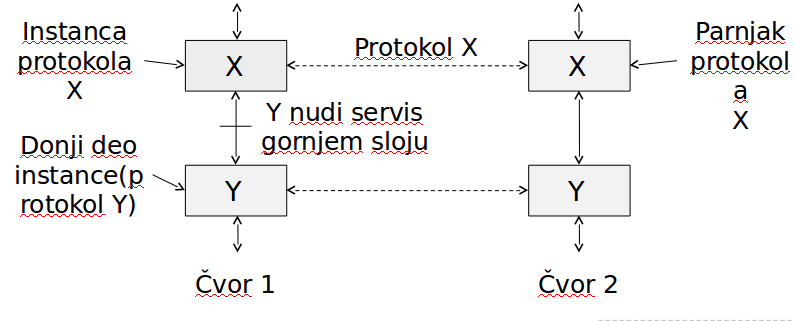
\includegraphics[width=9cm, height=5cm]{protokoli}\\
\end{center}

\subsection{Enkapsulacija}
Enkapsulacija je mehanizam slaganja slojeva protokola. Niži sloj pravi omotač oko sadržaja višeg sloja i dodaje svoje sopstvene informacije poruci. Sadržaj nižih slojeva je bliži spoljašnosti poruke. \\
\begin{center}
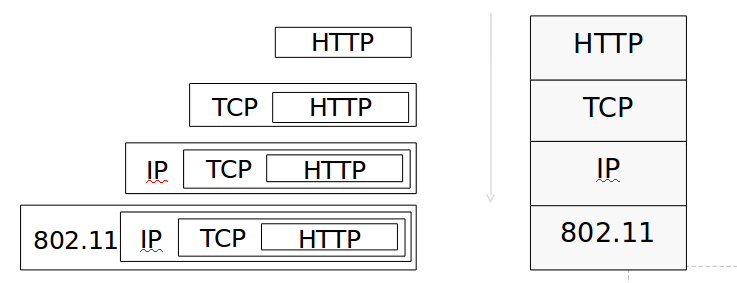
\includegraphics[width=9cm, height=4cm]{enkapsulacija}\\
\end{center}
Zahtev koji HTTP protokol definiše šalje se nižem sloju. TCP protokol dodaje svoja zaglavlja i skup informacija (metainf.) postaje sve veći kako se spuštamo po slojevima (to su enkapsulirane informacije). Zaglavlje sadrži upravljačke podatke, npr. zaglavlje jednog sloja može da sadrži redne brojeve koji omugućavaju tom istom sloju na drugom računaru da poruke isporuči ispravnim redosledom, za slučaj da niži slojevi taj redosled ne poštuju. Mogu da sadrže i veličine, vremena i druga polja. Sa svim tim informacijama se na poslednjem sloju poruka šalje na drugu stranu. Sad se informacije otpakuju, tj. primenjuje se inverzna funkcija za svaki od slojeva (uklanja se zaglavlje za svaki od slojeva) i kad se stigne do HTTP-a, on rekonstruiše originalnu poruku. \\
Smer toka podataka: $ \downarrow $(spušta se niz slojeve), zatim $ \rightarrow $
(prenosi se na najnižem sloju), pa $ \uparrow $ (podiže se uz slojeve).
\\
Protokol stek mora da bude poznat drugoj strani da bi bilo poznato kako treba da se otpakuje i svaki protokol zna samo svoju inverznu funkciju. Na drugoj strani, kada se poruka otpakuje, eliminišu se zaglavlja na svakom od slojeva i to se zove davanje usluge višim slojevima.\\
 Kada je nepogodno ili skupo da se za svaki par proces koji međusobno komuniciraju uspostavlja zasebna veza, odgovarajući sloj može da istu vezu upotrebi za više istovremenih, nezavisnih konverzacija. Sve dok je ovo \textit{multipleksiranje i demultipleksiranje} nevidljivo, može ga koristiti svaki sloj. Multipleksiranje je neophodno u fizičkom sloju gde se saobraćaj za sve veze mora preneti preko najviše nekoliko fizičkih linija. (kod njega na slajdovima stoji nešto za demultipleksiranje!)
 \\
\subsection{Prednosti raslojavanja}
- Prikrivanje informacija i ponovna upotreba\\
- Povezivanje različitih sistema\\
Šta se dešava ako imamo različite protokole na jednoj i na drugoj strani? Primer je slanje poruke sa uređaja zakačenog na WiFi na uređaj zakačenn na Ethernet. Tada na najnižim slojevima postoje tablice preslikavanja protokola. Poruka se samo prepakuje na poslednjem nivou. \\
\subsection{Mane raslojavanja}
- Povećani troškovi memorije i obrade (overhead)\\
Košta nas da dodajemo metapodatke. Manje bitno za duže poruke jer ne moramo svaki paket da dekorišemo. Početni i poslednji paket imaju veći broj informacija od središnjih, ali svaki paket ima dovoljno informacija da stigne na drugu stranu. Ne mora da budu početni i poslednji paket paketi koji imaju više informacija, mogu to biti i neki specijalni paketi. \\
- Prikrivanje informacija\\
Generalno je korisno, ali neke aplikacije žele da znaju da li se informacije prenose bežično ili putem kabla.


\section{Referentni modeli protokola i slojeva, jedince podataka, organizacije za standarde}
Ključno pitanje dizajna modela jeste koje funkcionalnosti implementira svaki od slojeva i koliko slojeva treba da postoji. Referentni modeli odgovaraju na ovakva pitanja. 
\subsection{OSI model sa 7 slojeva}

Internacionalan standard za povezivanje sistema. Uticajan ne, ali ne previše korišćen u praksi.
\\\\
1. \textbf{Fizički sloj}\\
Ima ulogu slanja \textit{bitova} putem realnih fizičkih komunikacionih kanala. U probleme njegovog projektovanja spada obezbeđivanje da kada jedna strana pošalje bit 1, druga strana takođe primi bit 1, a ne bit 0.\\\\
2. \textbf{Sloj veze podataka}\\
Ima ulogu slanja \textit{okvira}, odnosno skupova podataka. Pošiljalac ulazne podatke deli na okvire podataka, najčešće od po nekoliko stotina do nekoliko hiljada bajtova i okvire šalje jedan za drugim. Ako je usluga pouzdana, primalac potvrđuje ispravan prijem svakog okvira šaljući pošiljaocu okvir za potvrdu.
Jedan od problema koji se javlja u ovom sloju jeste neusaglašenost brzine slanja i brzine primanja podataka.\\\\
3. \textbf{Mrežni sloj}\\
Ima ulogu adresiranja, rutiranja \textit{paketa} i kontrole saobraćaja. Pri njegovom projektovanju ključno je odrediti kako se paketi upućuju od izvora ka odredištu. Putanje se mogu zasnivati na statičnim tabelama koje su ugrađene u mrežu i retko se menjaju. Jedan od zadataka ovog sloja je da omogući povezivanje heterogenih mreža.\\\\
4. \textbf{Transportni sloj}\\
Ima ulogu dostavljanja \textit{segmenata} (segmentacija, potrvđivanje). Osnovni zadatak je da prihvata podatke odzgo i da ih po potrebi razvrstava u manje grupe i da ih prosleđuje mrežnom sloju, obezbeđujući da svi delovi ispravno stignu na odredište. On takođe definiše usluge koje se nude sloju sesije.\\\\
5. \textbf{Sloj sesije}\\
Ima ulogu upravljanja sesijama.Omogućava korisnicima na različitim računarima da međusobno uspostave sesiju. Sesije nude različite usluge, uključujući upravljanje dijalogom, tj. vođenje računa o tome na koga je red da šalje poruke, rad sa žetonima, tj. sprečavanje učesnika da istovremeno pokrenu istu kritičnu operaciju i sinhronizovanje, tj. proveravanje dugačkog niza podataka tokom prenosa da bi se omogućilo nastavljanje od tačke prekida u slučaju pada sistema.\\\\
6. \textbf{Sloj prezentacije}\\
Ima ulogu konverzija za različite prezentacije. Bavi se sintaksom i semantikom prenetih informacija. Da bi računari koji podatke predstavljaju na različit način mogli da komuniciraju, strukture podataka koji se prenose mogu se definisati na apstraktan način i standardno kodirati u cilju prenosa. Sloj prezentacije obrađuje te apstraktne strukture podataka.\\\\
7. \textbf{Sloj aplikacije}\\
Ima funkcije potrebne korisniku, rad sa \textit{porukama}.  
\\
\\
Mana ovog modela jeste to što su  slojevi sesije i prezentacije gotovo prazni dok su sloj veze podataka i mrežni sloj prenatrpani.


\subsection{Internet referentni model}
Model sa 4 sloja, zasnovan na praksi. Sva tri gornja sloja se stapaju u jedan.
1. \textbf{Veza}\\
Ima ulogu fizičkog slanja podataka putem medijuma.Sam protokol za povezivanje s mrežom nije definisan i menja se od računara do računara i od jedne mreže do druge. \\\\
2. \textbf{Internet}\\
Ima ulogu slanja paketa putem raznorodnih mreža. Definiše Inernet protokol. Zadatak je da isporuči IP pakete tamo gde treba da stignu. Ovde je najveći problem problem usmeravanja i izbegavanja zagušenja.\\\\
3. \textbf{Transport}\\
Ima ulogu razmene podataka između čvorova. On je namenjen konverzaciji između ravnopravnih procesa na izvornom i odredišnom računaru, kao i transportni OSI sloj. Ovde su definisana dva protokola, protokol za upravljanje prenosom - TCP i protokol za korisničke datagrame - UDP. \\
TCP je pouzdan protokol sa uspostavljanjem direktne veze. Deli početni tok bajtova na zasebne poruke i svaku prosleđuje međumrežnom sloju. Prihvatni TCP proces na odredištu uređuje primljene poruke i od njih ponovo obrazuje tok bajtova. On upravlja i tokom podataka tako da brzi pošiljalac ne može da zatrpa sporog primaoca s više poruka nego što ovaj može da obradi. \\
UDP  predstavlja nepouzdan protokol bez uspostavljanja direktne veze namenjen aplikacijama koje same uređuju svoje pakete i upravljaju tokom podataka.\\\\
4. \textbf{Aplikacija}\\
Programi koji koriste usluge mreže. Sadrži sve protokole višeg nivoa - FTP za prenos datoteka, SMTP za elektronsku poštu, TELNET za virtuelni terminal koji omugućava korisniku da se sa svog računara daljinski prijavi na drugi računar i da na njemu radi, DNS za imenovanje domena, tj. za preslikavanje imena računara u njihove mrežne adrese, HTTP protokol za preuzimanje strana sa Worl Wide Weba i mnogi drugi.
\\\\
IP sloj je najtanji po pitanju broja protokola.

\begin{center}
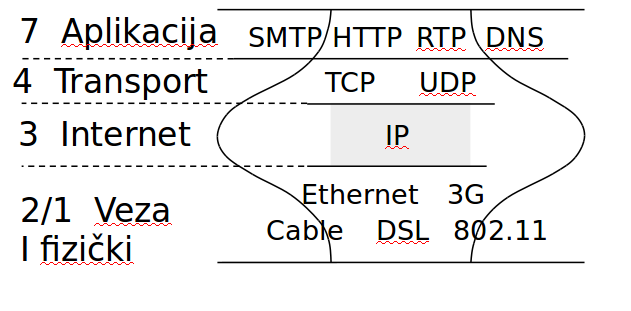
\includegraphics[width=9cm, height=4cm]{InternetRefModel}\\
\end{center}

Mana ovog modela jeste da on nije dovoljno uopšten, na primer, opisati Bluetooth pomoću ovog modela je sasvim nemoguće. Još jedna mana je to što ne razdvaja fizički sloj i sloj veze podataka. Ta dva sloja su potpuno različita. \\
\\

Mi ćemo koristiti hibridni model sa 5 slojeva: fizički sloj (bit), sloj veze (okvir), mrežni sloj (paket), transportni (segment) i aplikativni sloj (poruka). Jedinice podataka za svaki od slojeve su navedene u zagradama.\\
\\
Nazivi nekih uređaja u mreži: \\
- hab ili razvodnik ponavlja fizički signal na sve izlaze\\
- svič ili skretnica usmerava pakete samo onima kojima su potrebni, znači čita adresu\\
- ruter ili usmerivač usmerava pakete ali vodi računa i o dobrim putanjama\\\\

Neke poznatije organizacije za standarde:\\

\begin{center}
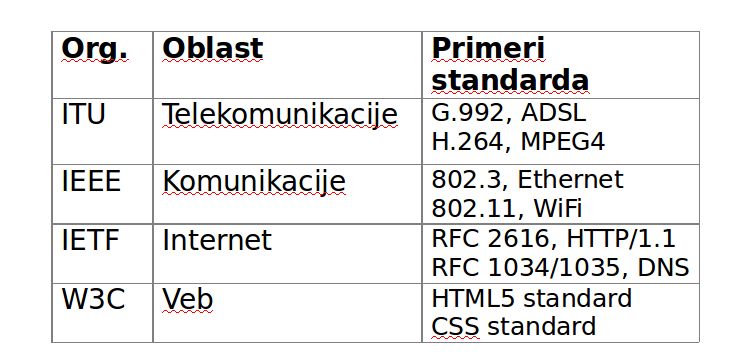
\includegraphics[width=9cm, height=4cm]{organizacije}\\
\end{center}
(Ovde kaže da treba i poglavlja 1.6 i 1.7, ali ja ne znam da li tu ima bilo šta bitno.)

\section{Fizički sloj, uloga, pojednostavljeni model, kašnjenja, BDP, primeri}
Tiče se slanja poruka putem komunikacionog kanala. Žice šalju analogni, tj. fizički signal, a mi želimo da šaljemo bitove koji su digitalni. Osnovna svrha je da niz bitova prenese bez greške s jednog računara na drugi. Za prenos mogu da se koriste različiti fizički medijumi. 
\subsection{Pojednostavljeni model}
Karakteristike uopštenog fizičkog kanala koje utiču na to koliko je kanal dobar:\\
- \textbf{\textit{protok}} (ili brzina, kapacitet) meren kao bitovi po sekundi b/s, označimo ga sa B\\
- \textbf{\textit{kašnjenje}} mereno u sekundama\\
Podrazumeva vreme potrebno da poruka stigne na ciljnu adresu. Označimo ga sa D. Postoje dve vrste kašnjenja, a to su: \\
1. \textit{Kašnjenje prenosa}, tj. vreme potrebno da se M-bitovna poruka postavi na komunikacioni kanal i različito je za sve kanale:
                 \begin{center}
                 T-delay = M (b) / B (b/s) = M/B s (sekundi)
                 \end{center}
2. \textit{Kašnjenje propagacije}, tj. vreme potrebno da bitovi prođu kroz komunikacioni kanal i slično je za sve kanale:
                  \begin{center}
           P-delay = dužina kanala/brzina signala (2/3 c) = X s (sekundi)
          *c – brzina svetlosti (nije svuda 2/3, različito za WiFi, optiku, ...)
                  \end{center}
Sabiranjem se dobija ukupno vreme.
                         \begin{center}
                         L = T+P = M/B + P
                         \end{center}
- \textbf{\textit{da li kanal emituje ili ne}}\\
- \textbf{\textit{raspodela verovatnoća grešaka}}\\
Primeri izračunavanja kašnjenja: \\
“Dialup” sa telefonskim modemom (slanje ka računaru u istom gradu npr):
                    \begin{center}
               P = 5 ms, B = 56 kb/s, M = 1250 B\\
              
               L = 5 ms + (1250x8)/(56 x 103) s = 5 ms+179 ms = 184 ms
                      \end{center}
Dugačka veza ili mali protok proizvode veće kašnjenje. Obično je jedna od komponenti kašnjenja P ili T dominantna.
\subsection{Protok-kašnjenje proizvod BDP}
BDP jeste proizvod protoka i vremena kašnjenja.
                     \begin{center}
                       BDP = B x D
                      \end{center}
Poruke zauzimaju prostor na kanalu. Količina podataka prisutnih na kanalu u nekom momentu je BDP. Ako bismo posmatrali podatak kao materiju, onda je ovo zapremina, tj. količina materije BDP = B x D. Meri se u bitovima i BDP je mali za kanale u lokalnim mrežama, npr. WiFi, a veliki za velike debele kanale.\\
\textbf{BDP primer}:\\
Slanje npr. od Perta do Sidneja preko optičkog kanala koji je dugačak.\\
B=40 Mb/s, D=50 ms $ \Rightarrow $ BDP = 40 x $10^{6}$ x 50 x $10^{-3}$ b = 2000 Kb = 250 KB\\
Ovo se smatra velikim BDP-om.\\
\\
Medijum propagira signal sa informacijama u vidu bitova. Tri osnovna tipa medija su: \\
- žičani\\
- optički (optički kablovi)\\
- bežični

\section{Žičani i optički komunikacioni medijumi}
Prednost je što se lako projektuje fiksni protok duž odabranih ruta, a mane su da je skup za postavljanje, posebno na većim udaljenostima i nije projektovan za mobilnost ili emitovanje.
\subsection{Žičani}
\subsubsection{Upredena parica}
Veoma česta, koristi se za LAN kablove i kod telefonskih linija.  Čine je dve izolovane bakarne žice, najčešće prečnika oko 1mm. Žice su međusobno spiralno uvijene, kao molekul DNK. Uvrtanjem se umanjuju smetnje. Najčešće se koristi u telefonskom sistemu, skoro svi telefoni su sa telefonskom centralom povezani uporednom paricom. Kada se veliki broj paralelnih parica protežu na veću daljinu, na primer sve linije iz jednog stambenog bloka do telefonske  centrale, one se povezuju u snop i obavijaju zaštitnim omotačem. Njome se mogu prenositi i analogni i digitalni signali. Brzina prenosa zavisi od debljine žice i rastojanja, ali se za daljine od nekoliko km u većini slučajeva može postići brzina od više megabita u sekundi.\\
Uporedna parica se realizuje u više oblika, od kojih su dva važna za računarske mreže. \\
- uporedna parica 3. kategorije se sastoji od dve blago uvijene izolovane žice. Četiri takva para obično se grupišu u zajedničkom plastičnom omotaču koji ih drži zajedno i štiti. \\
- uporedna parica 5. kategorije koje liče na parice 3. kategorije, ali su gušće upredene, čime je omogućen kvalitetniji signal na većim razdaljinama zbog čega su pogodnije za brzu komunikaciju između računara. \\
Uporedna parica 5. kategorije:
\begin{center}
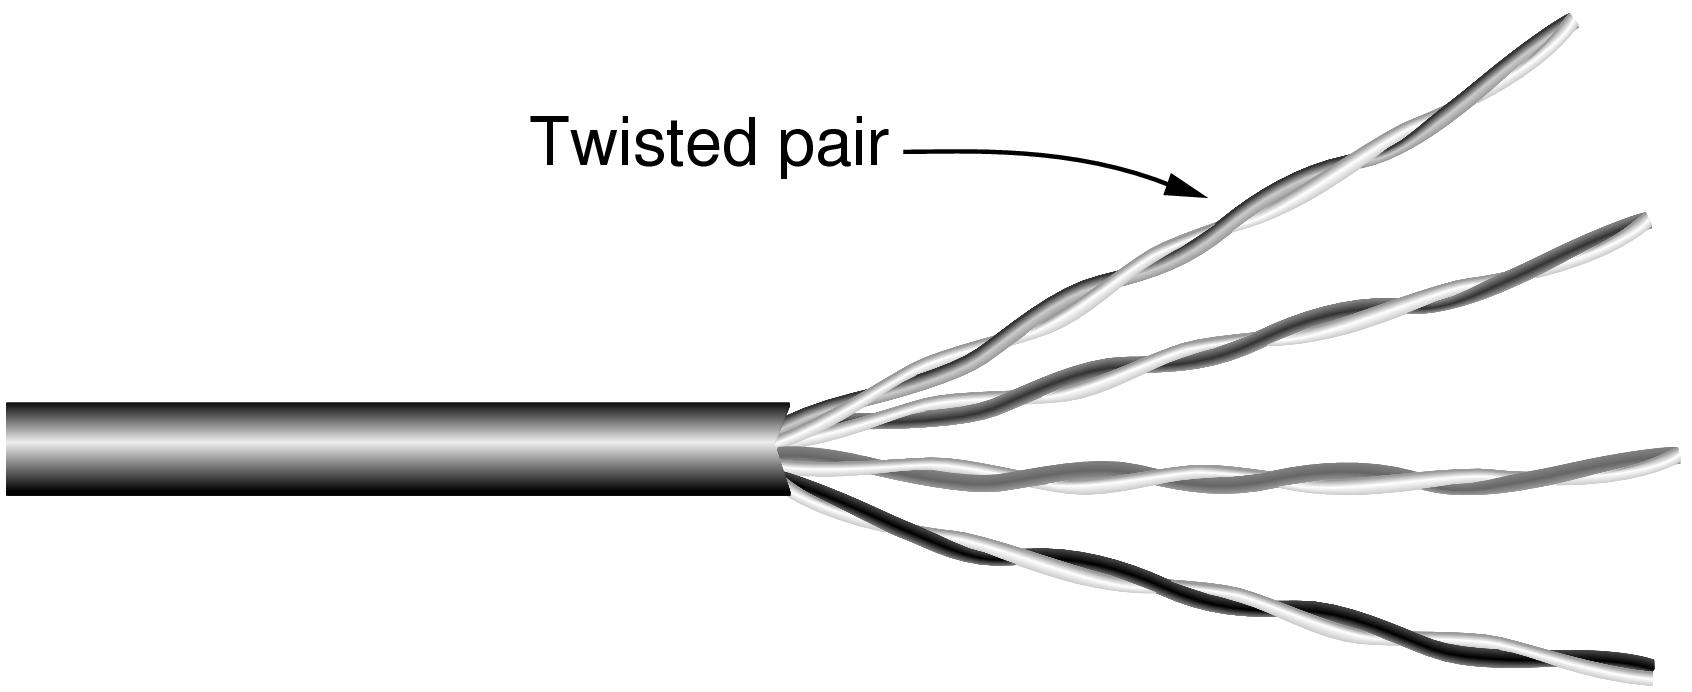
\includegraphics[width=7cm, height=3cm]{parica}\\
\end{center}

\subsubsection{Koaksijalni kabl}
Takođe čest. Daje bolju zaštitu i bolje performanse. Podatke prenosi većom brzinom i na veće daljine u odnosu na uporedne parice. Koriste se 50-omski i 75-omski koaksijalni kabl. Prvi se namenjuje digitalnom prenosu podataka, a drugi se koristi za prenos analognih podataka i za kablovsku televiziju, ali postaje sve važniji i za kablovski Internet. \\
Ovaj kabl ima jezgro od čvrste bakarne žice oko koje se nalazi izolator. Oko izolatora je cilindrični provodnik napravljen od gusto upletene bakarne mrežice. Preko njega dolazi zaštitni plastični omotač. Presek koaks. kabla:
\begin{center}
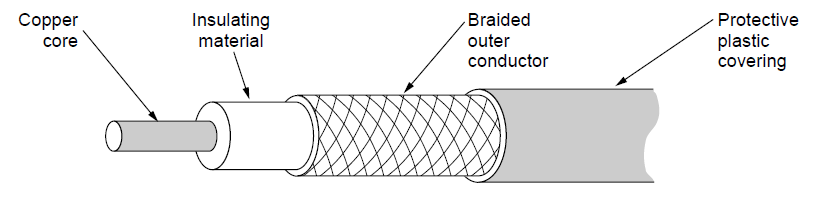
\includegraphics[width=12cm, height=3cm]{koaksijalni}\\
\end{center}
Savremeni koaks. kablovi imaju propusni opseg blizu 1GHz. Ranije su mnogo korišćeni za međugradske i međudržavne veze u telefonskim sistemima, ali su danas tu većinom zamenjeni optičkim kablovima. I dalje se koriste za kablovsku televiziju i gradske mreže.
\subsubsection{Instalacije za prenos struje}
Praktične za upotrebu jer već postoje. Jako loše karakteristike prenosa jer nisu dizajnirane za to.
\begin{center}
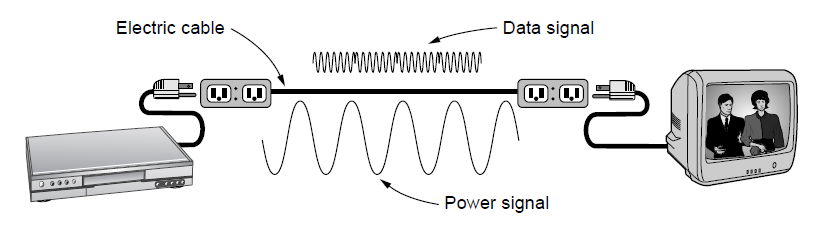
\includegraphics[width=12cm, height=3cm]{zicani}\\
\end{center}

\subsection{Optički}
Dugačka, tanka i čista vlakna stakla. Ogroman protok zbog opsega frekvencija. Velike udaljenosti zbog malog slabljenja. \\
Optički sistem za prenos podataka sadrži tri glavne komponente: svetlosni izvor, prenosni medijum i detektor. Po konvenciji, svetlosni impuls označava bit 1, a odsustvo impulsa označava bit 0. Prenosni medijum je ultratanko stakleno vlakno. Detektor proizvodi električni impuls kada na njega padne svetlosni zrak. Spajajući svetlosni izvor s jednim krajem optičkog vlakna, a detektor sa njegovim drugim krajem, dobijamo jednosmerni sistem prenosa podataka koji prihvata električni signal, pretvara ga u svetlosni impuls i prenosi, a zatim ga na drugom kraju pretvara u električni signal.
\begin{center}
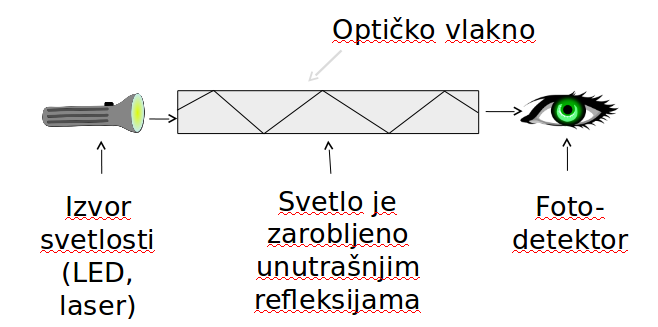
\includegraphics[width=9cm, height=4cm]{opticki1}\\
\end{center}
 Kada upadni ugao zraka pređe određenu kritičnu vrednost, zrak uopšte ne prelazi u vazduh, već se vraća u kvarc. Na taj način je zauvek zarobljen u vlaknu.\\
Slabljenje svetlosti pri prolasku kroz staklo zavisi od talasne dužine svetlosti, a i od izvesnih svojstava stakla. \\
Optički kablovi su slični koaks. kablovima samo što nemaju mrežasti provodnik.  Duž ose kabla proteže se stakleno jezgro kroz koje prolazi svetlosni zrak. Jezgro je okruženo oblogom od stakla čiji je indeks prelamanja manji od indeksa prelamaja jezgra kako bi se sva svetlost zadržala u jezgru. Oko svega se nalazi plastični omotač koji štiti oblogu. Vlakna se najčešće grupišu u snopove i zaštićuju dodatniim spoljim omotačem.
Koriste se za lokalne mreže i za prenos podataka na velika rastojanja. Polažu se na dubini od jednog metra ispod površine tla.\\

Pojedinačno vlakno i pakovanje vlakna:
\begin{center}
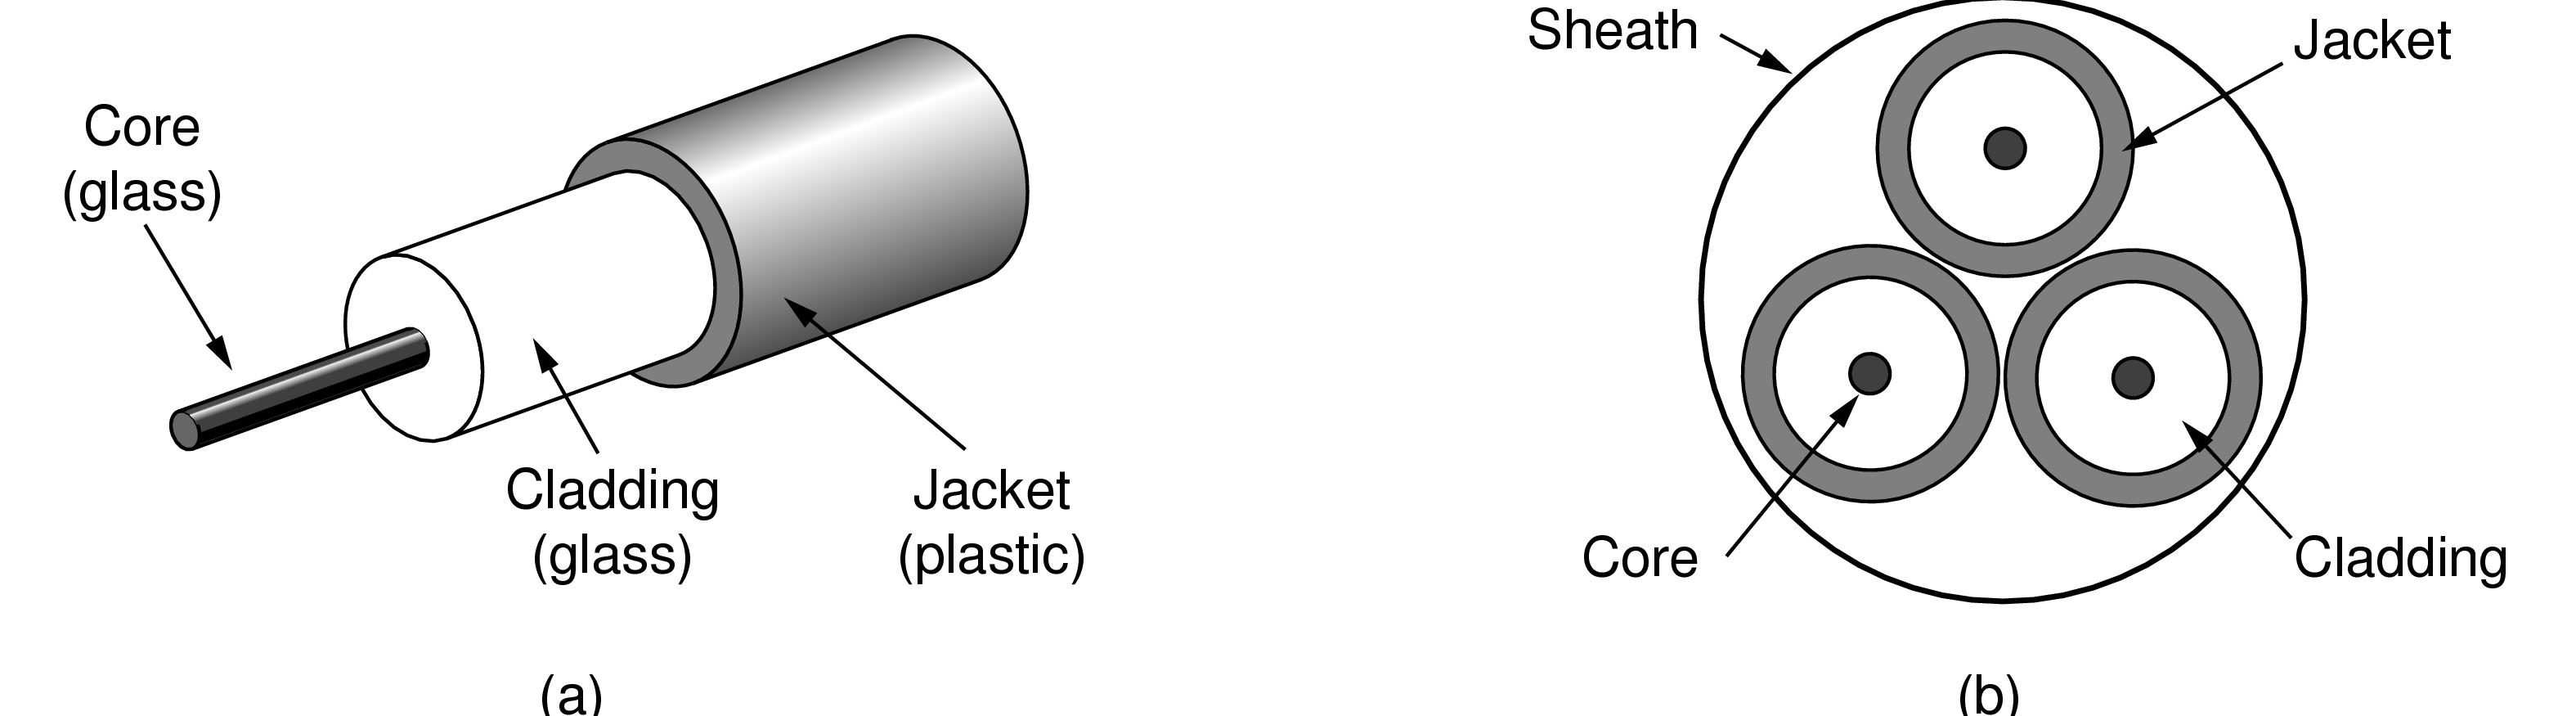
\includegraphics[width=12cm, height=3cm]{pojedinacno}
\end{center}

\subsubsection{Unimodalno vlakno}
Toliko je tanko da svetlost praktično ide pravo. Vlakno radi kao talasovod i svetlost se kroz njega prostire pravolinijski, bez odbijanja. Drugi naziv je jednorežimsko vlakno. Skuplja su od višerežimskih i koriste se za veća rastojanja. Mogu da prenose signale na daljinu od 100km, brzinom 50 Gb/s.
\begin{center}
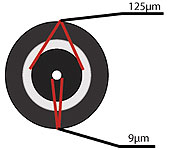
\includegraphics[width=3cm, height=2cm]{unimodalno}\\
\end{center}

\subsubsection{Višemodalno vlakno}
Kod ovog vlakna svetlost se sudara sa zidovima. Kroz vlakno može istovremeno prolaziti više svetlosnih zrakova od kojih se svaki odbija pod drugačijim uglom, uvek većim od kritične vrednosti. Za svaki zrak se kaže da kroz vlakno prolazi drugačijim režimom, pa se zbog toga zovu višemodalna ili višerežimska vlakna.
\begin{center}
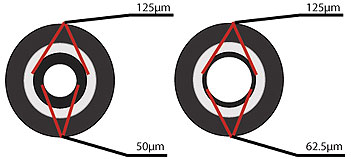
\includegraphics[width=5cm, height=2cm]{visemodalno}\\
\end{center}

\section{Bežični komunikacioni medijumi}
Prednosti su da prirodno podržavaju emitovanje, jednostavne za postavljanje i jeftine, prirodno podržavaju mobilnost, a mane su mešanje signala koje se mora razrešavati i to što jačina signala, pa samim tim i protok, izuzetno varira.\\
Pošiljalac emituje signal kroz prostor. Signal se emituje u svim pravcima za razliku od žice. Bliski signali, tj. signali slične frekvencije, se mešaju kod primaoca, pa je potrebno koordinirati upotrebu. Kako bi se izbegla mešanja signala, opsezi, tj. bandovi se pažljivo dodeljuju. Čak se prodaju na aukcijama za najviše ponude.\\
Za mreže je najinteresantniji opseg mikrotalasa (3G, 4G, WiFi), ali se koriste i ostali delovi spektra.\\
\begin{center}
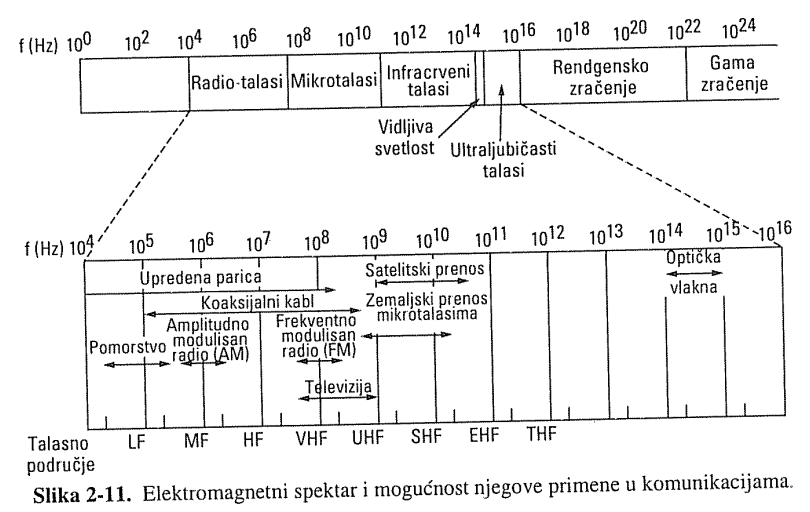
\includegraphics[width=10cm, height=6cm]{eltalasi}\\
\end{center} 
Drugačiji pristup od dodeljivanja frekvencija je da se one uopšte ne dodeljuju. Pusti se da svako po volji emituje, ali da se snaga emitovanja ograniči na mali radijus da emisije ne ometaju jedna drugu. U tom smislu, većina zemalja je odvojila određena talasna područja, zvana \textbf{industrijska, naučna i medicinska frekvencija} (\textit{Industrial, Scientific, Medical - ISM}) za nelicencirano korišćenje. Daljinski upravljači za garažna vrata, bežični telefoni, igračke i brojni drugi bežični kućni aparati koriste ISM područja.\\
Mikrotalasi, 3G i nelicencirane frekvencije (ISM) - obično zbog fragmentacije drugih bandova, npr. WiFi. (???? uzeto sa slajdova). Slika dole se odnosi na ovo.
\begin{center}
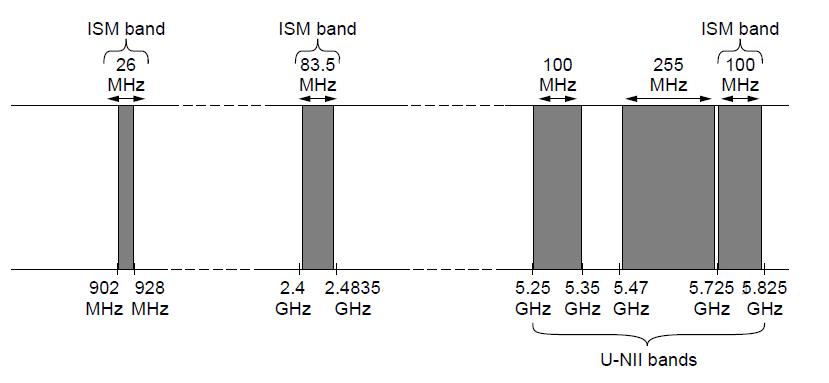
\includegraphics[width=10cm, height=4cm]{stagod}\\
\end{center} 

\subsection{Radio-talasi}
Radio-signali mogu da prolaze kroz zgrade, ali im signal slabi iz raznih razloga. Neki od razloga su to što biva apsorbovan ili zbog odbijanja. U opsezima VLF(very low freq.), LF(low freq.) i MF(medium freq.) radio-talasi prate zakrivljenost zemlje (ovi talasi lako prolaze kroz zgrade što omogućuje da se u njima slušaju tranzitorski prijemnici), a u HF(high freq.) opsegu se odbijaju od jonosfere i vraćaju se nazad, na Zemlju (što se koristi za komunikaciju radio-amatera na velikim rastojanjima). Radio-talasi se prostiru na sve strane od izvora, tako da položaj predajnika i prijemnika nije od velikog značaja.
\subsection{Mikrotalasi}
Imaju veliki frekventni opseg i koriste se često za zatvorene namene poput WiFi, kao i za otvorene poput 3G i sateliti. Mikrotalasi su talasi na frekvenciji iznad 100 MHz. Pošto se mikrotalasi prostiru pravolinijski (sva energija se koncentrise u uzak snop pomoću patabolične antene), zbog zakrivljenosti Zemlje, tornjevi ne smeju biti previše udaljeni. Što su tornjevi viši, rastojanje između njih može da bude veće. Mikrotalasi loše prolaze kroz zidove. Signal slabi i reflektuje se od objekata iz okruženja. Jačina varira zbog udaljenosti, sabiranja signala i slično. I kada se talasi dobro usmere na predajniku, oni se ipak na putu mogu rasuti. Neki talasi se mogu odbiti od niskih atmosferskih slojeva i zato na cilj stići kasnije od direktnih talasa. Zakasneli talas može da dođe u suprotnu fazu s direktnim talasom i da ga tako poništi. Taj efekat se zove \textit{slabljenje zbog različitih putanja}.
\subsection{Svetlost}
Svetlosni signali (ne misli se na optička vlakna) se mogu koristiti kao komunikacioni medijum. Svetlost je vrlo usmeren talas i ima veliki frekventni opseg (protok u elektroinženjerskom smislu).\\
Koristi se za povezivanje lokalnih mreža u dve zgrade pomoću laserskih uređaja na krovovima. Laserski zrak je po prirodi usmeren, tako da na svakoj od dve zgrade mora postojati i laser i fotodetektor. Takav sistem ima veoma veliku propusnu moć i izuzetno je jeftin. Za njega nije potrebno tražiti zvaničnu dozvolu vlasti, za razliku od mikrotalasa. \\
Nedostatak je što moć laserskog snopa ne može da prodre kroz kišu ili maglu, ali tokom sunačnih dana on radi odlično.
\begin{center}
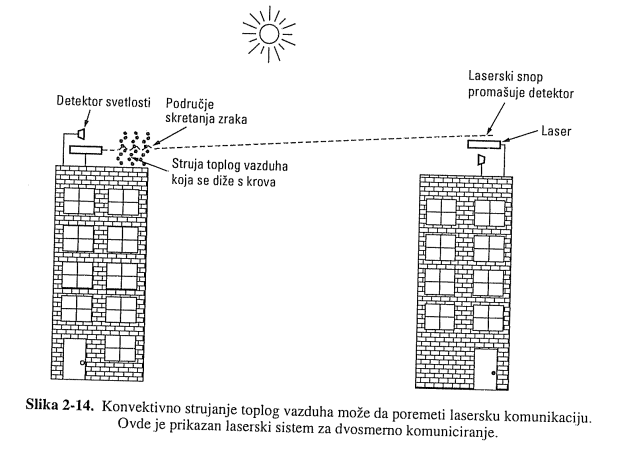
\includegraphics[width=12cm, height=8cm]{svetlost}\\
\end{center}

\section{Komunikacioni sateliti}
Sateliti su efikasni za emitovanje i komunikaciju bilo kada i bilo gde. \\
Kom. satelit može da se zamisli kao veliki repetitor na nebu koji sadrži više transpondera od kojih svaki osluškuje određeni deo elektromagnetnog spektra, pojačava primljeni signal i ponovo ga emituje na drugoj frekvenciji. \\
Tipovi satelita:
\begin{itemize}
  \item Geostacionarni (GEO)
  \item Srednje-orbitni (MEO)
  \item Nisko-orbitni (LEO)
\end{itemize}
\begin{center}
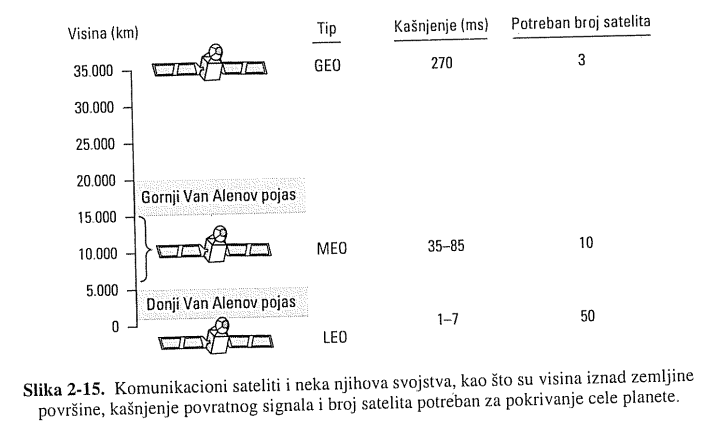
\includegraphics[width=12cm, height=8cm]{sateliti}\\
\end{center}
\subsection{Geostacionarni sateliti}
Orbitiraju 35000km iznad fiksne lokacije. Najnovije dostignuće na ovom polju jesu jeftine mikrostanice - \textbf{terminali s vrlo uskim emisionim snopom} (\textit{Very Small Aperture Terminals, VSATs}). U mnogim VSAT sistemima, mikrostanice nemaju dovoljnu snagu da direktno komuniciraju jedna s drugom (preko satelita), već se saobraćaj između njih odvija preko tzv. habova, ili razvodnika - zemaljske antene visokog učinka. VSAT dobija i šalje signal ka centralnom uređaju koji se naziva hab (postoje i sistemi bez centralizovanog uređaja). Hab, na primer, odašilja televizijski program ka GEO, a ovaj emituje na delu zahvaćene Zemljine teritorije, te ka svim pripadajućim VSAT uređajima. U ovakvom režimu rada, korišćenjem mikrostanica male snage, kašnjenje signala je veće.\\
\begin{center}
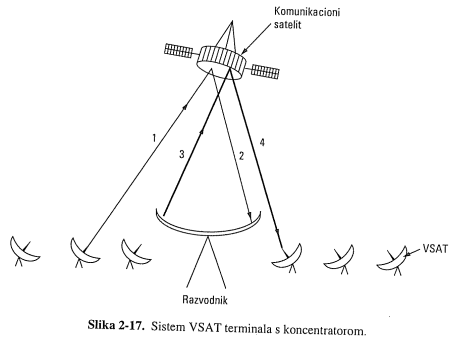
\includegraphics[width=12cm, height=8cm]{GEO}\\
\end{center}
Svojstvo satelitskog prenosa je i to što cena prenete poruke ne zavisi od udaljenosti. Prekookeanska veza košta kao i veza sa komšijom preko puta. Sa aspekta bezbednosti i privatnosi, sateliti su jako loši jer svako može sve da čuje. Neophodno je šifrovati podatke.
\subsection{Nisko-orbitni sateliti}
Nisu geostacionarni pa zbog toga što se brzo kreću mora da ih ima više kako bi mogli da garantuju stalnu pokrivenost na odabranim regijama. Brži odziv u odnosu na GEO jer su bliži Zemlji (kašnjenje signala iznosi nekoliko milisekundi). \\
\begin{center}
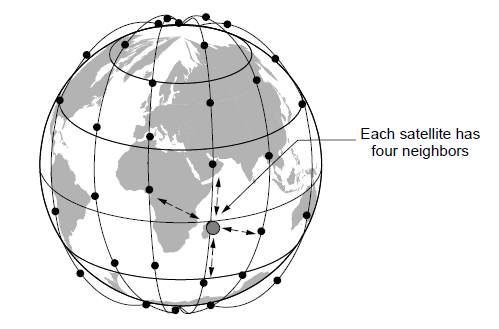
\includegraphics[width=8cm, height=5cm]{LEO}\\
\end{center}
Jedna vrsta ovakvih sistema je namenjena Internetu, a to je \textbf{Teledesic}. Cilj sistema bio je da se za milione korisnika Interneta obezbedi istovremena veza ka satelitu brzine do 100Mb/s, a od satelita do 720Mb/s. 
\subsection{Sateliti ili optika?}
Prednosti satelita su:
\begin{itemize}
  \item nakon lansiranja satelita, komunikacija može brzo da se uspostavi bilo gde i bilo kada
  \item emitovanje na velika područja
\end{itemize} 
Mane satelita su:
\begin{itemize}
  \item ograničen protok
  \item mešanje signala
\end{itemize}
Prenosti optike:
\begin{itemize}
  \item ogroman protok duž velikih udaljenosti
\end{itemize}
Mana optike:
\begin{itemize}
  \item instalacija skupa
  \item instalacija komplikovana
\end{itemize}

\section{Signali, prenos, frekvenciona reprezentacija, signal u žičanim, optičkim, bežičnim medijumima}
(pogledati knjigu 2.1.1 i 2.1.2 poglavlja)\\

Analogni signali kodiraju digitalne. Šta se dešava sa signalom prilikom propagacije?\\
Podaci se mogu prenositi žicom tako što se menja neko njeno fizičko svojstvo, npr. napon ili jačina struje. Kada predstavimo vrednost tog napona ili te jačine struje kao jednoznačnu funkciju vremena, f(t), možemo da modeliramo ponašanje signala i da ga analiziramo služeći se matematičkim metodama. \\

Signal se kroz vreme može predstaviti putem svojih frekvencijskih delova (Furijeova analiza).\\
Svaka normalna periodična funkcija $ g(t) $ periode $ T $ se može predstaviti kao zbir (možda beskonačnog) broja sinusnih i kosinusnih funkcija:
\begin{center}
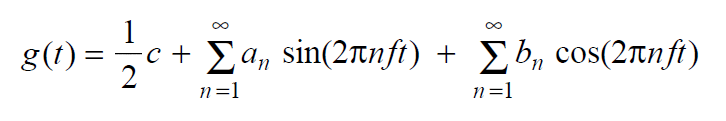
\includegraphics[width=10cm, height=2cm]{furije}\\
\end{center}
gde je $ f = 1/T $ osnovna frekvencija, $ a_{n} $ i $ b_{n} $ su amplitude $ n$-tog člana (harmonika) sinusne i kosinusne funkcije, a $c$ je konstanta. Tako razložena periodična funkcija naziva se \textbf{Furijeov niz}. Iz njega se može rekonstruisati prvobitna funkcija; to znači, ako je poznata perioda $T$ i ako su zadate amplitude prvobitna funkcija se dobija sabiranjem niza iz gornje jednačine.\\

Signal podataka koji ima ograničeno trajanje može se rastaviti u Furijeov niz ako zamislimo da se njegov profil stalno ponavlja, tj. da se profil iz intervala $0$ do $T$ istovetno ponavlja u intervalu od $T$ do $2T$, itd.\\

Amplitude $a_{n}$ mogu se izračunati za svaku funkciju $g(t)$ množenjem obe strane gornje jednačine činiocem $sin(2 \pi kft)$, a zatim integrisanjem jednačine u intervalu od $0$ do $T$. Slično tome, množeći gornju jednačinu sa $cos(2 \pi kft)$ i integrišući je između $0$ i $T$, možemo da dobijemo amplitudu $ b_{n} $. Neposrednom integracijom obe strane gornje jednačine  dobijamo $c$.
\begin{center}
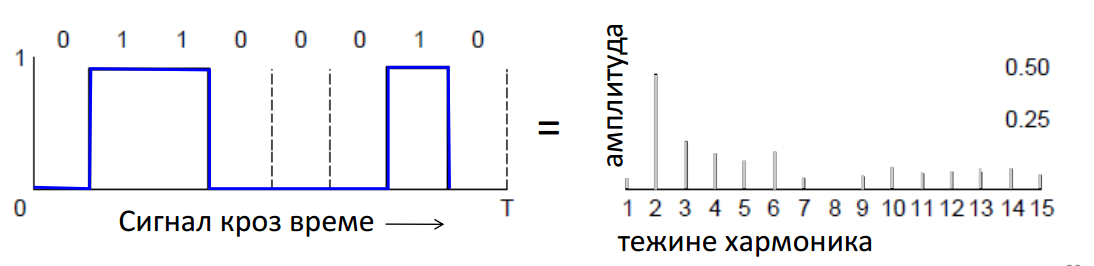
\includegraphics[width=12cm, height=3cm]{furije2}\\
\end{center}

Da bismo razumeli kakve veze ovo ima s prenosom podataka, razmotrimo jedan primer: slanje slova $b$ kodiranog pomoću 8 bitova. Niz bitova koje treba preneti izgleda ovako: 01100010. Leva strana gornje slike prikazuje napon signala koji šalje računar. Srednjekvadratne amplitude, za prvih nekoliko članova niza, prikazane su na desnoj strani slike. One su važne jer su njihovi kvadrati proporcionalni energiji koja se pri određenoj frekvenciji prenese. \\

Nema transportnog medijuma koji prenosi signale bez gubitaka. Kada bi sve komponente Furijeovog niza podjednako slabile, amplituda signala bila bi takođe manja, ali se signal ne bi izobličio, tj. imao bi isti pravougaoni oblik kao na gornjoj slici. Nažalost, u svim prenosnim medijumima različite komponente F. niza različito slabe, što dovodi do izobličenja signala. Opseg frekvencija koje se prenose bez većeg slabljenja naziva se \textbf{propusni opseg}. Često se definiše kao opseg frekvencija od 0 do frekvencije pri kojoj snaga signala opadne na polovinu.
\\

Manji skup frekvencija, manji protok:
\begin{center}
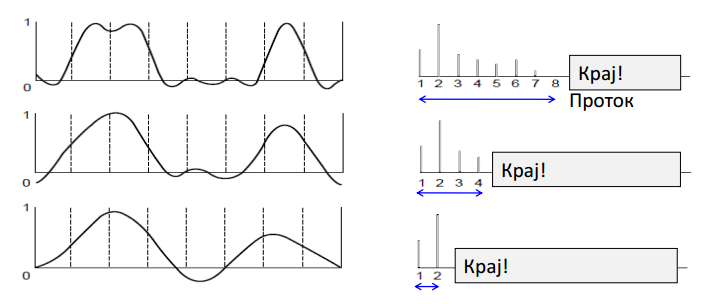
\includegraphics[width=12cm, height=6cm]{furije3}\\
\end{center}

Ograničavanjem propusnog opsega ograničava se i brzina prenosa, čak i kroz savršene kanale.\\
Elektroinženjeri: Protok  je širina frekv. opsega (Hz)\\
Računarci: Protok je kapacitet prenosa informacija (b/s)

\subsection{Signal preko žice}
Šta se dešava sa signalom dok prelazi kroz žicu?
\begin{itemize}
  \item signal kasni (brzina je ~$2/3c$, a ne beskonačna)
  \item signal slabi (sa porastom udaljenosti)
  \item frekvencije iznad neke granice brže slabe
  \item dešava se šum (zbog spoljnih efekata)
\end{itemize}
\begin{center}
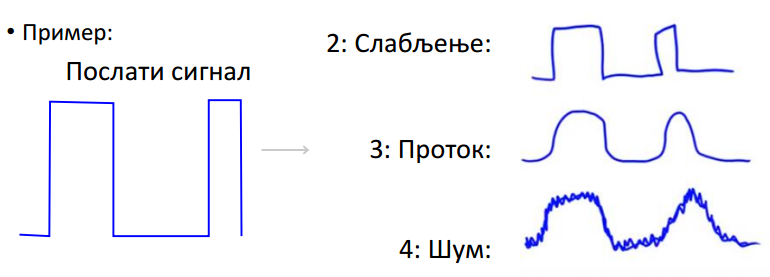
\includegraphics[width=15cm, height=5cm]{protok1}\\
\end{center}

\subsection{Signal preko optike}
Svetlo se prenosi sa veoma malim gubitkom u tri široka frekventna opsega. Krajni desni zalazi u opseg infracrvenih talasa.
\begin{center}
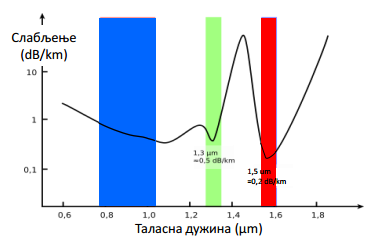
\includegraphics[width=8cm, height=5cm]{protok2}\\
\end{center}

\subsection{Signal u bežičnim komunikacijama}
Zbog visokih frekvencija bežičnih prenosa, nije moguće digitalni signal direktno kodirati u analogni, već se koristi koncept \textbf{signala nosača}.
\begin{center}
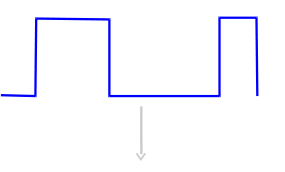
\includegraphics[width=3cm, height=2cm]{signal}\\
\end{center}
\begin{center}
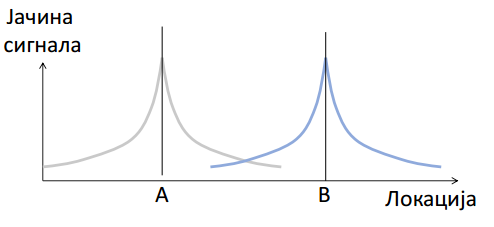
\includegraphics[width=6cm, height=3cm]{signal2}\\
\end{center}
Putuje brzinom svetlosti, ali jako brzo slabi (sa kvadratom rastojanja, zašto?)\\

Višestruki signali na istoj frekvenciji se mešaju kod primaoca. Ako su lokacije dovoljno udaljene, moguće je koristiti istu frekvenciju.
\begin{center}
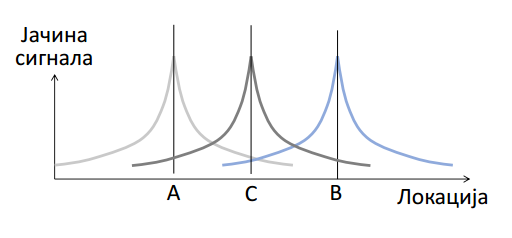
\includegraphics[width=6cm, height=3cm]{signal3}\\
\end{center}
Postoje još neki otežavajući efekti. Propagacija bežičnog signala je složena i zavisi od okruženja. Karakteristike zavise i od frekvencije. Ne prenosi se isto zvuk i svetlost, u čemu je razlika? Postoji problem sa \textit{sabiranjem odbijenih signala} kod mikrotalasa. Signali mogu da se odbijaju od objekta i putuju kroz više nezavisnih putanja. Posle, kada stignu višestruki signali kod primaoca, oni se mogu loše sabrati.  Primer:
\begin{center}
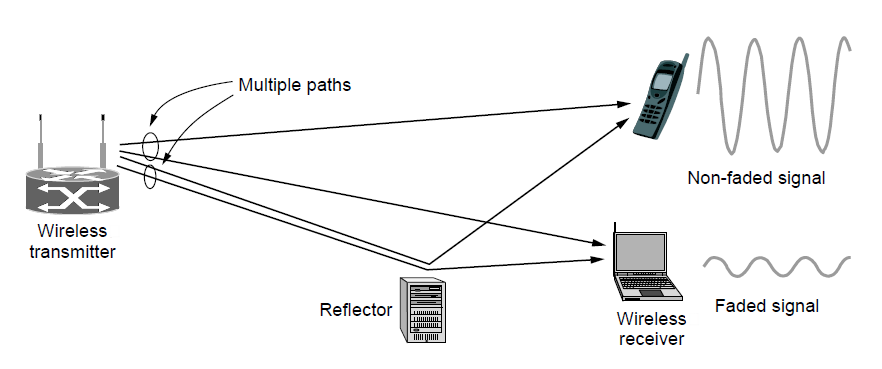
\includegraphics[width=10cm, height=4cm]{signal4}\\
\end{center}

\section{Modulacija i multipleksiranje signala}
Sa slajdova i u knjizi poglavlje.


\section{Prirodna ograničenja prenosa signala}
Čak i savršen kanal ima ograničen kapacitet prenosa.
Koliko često se može slati podatak kroz kanal? O tome govore Najkvistov limit i Šenonov kapacitet. Realni sistemi su dobro realizovani ako nisu mnogo daleko od ovih ograničenja. Ograničenja nam govore koliko smo relativno dobri u nečemu.\\
Protok - B, jačina, tj. snaga signala - S, jačina, tj. snaga šuma - N. B ograničava brzinu promena - frekvenciju i to je karakteristika kanala. S i N ograničavaju broj razlučivih nivoa signala i to je karakteristika primaoca.\subsection{Najkvistov limit}
Maksimalan broj promena simbola je 2B (101010101010101010..). Ako postoji V nivoa signala (ignorišemo greške, tj. šum), onda je maksimalan protok u bitima, tj. najveća brzina prenosa:
\begin{center}
 $ R=2B log_{2} V$  b/s.
\end{center}
Ovo je jednačina za maksimalnu brzinu prenosa kroz bešumni kanal ograničene propusne moći. \\
Na primer, bešumni kanal propusnog opsega 3 kHz ne može da prenosi binarne signale brzinom većom od 6000 b/s.

\subsection{Šenonov kapacitet}

Proširenje Najkvistove jednačine na kanale sa slučajnim, tj. termičkim šumom. Termički šum uvek postoji zbog kretanja molekula u sistemu. Izražava se kao količnik snage signala i snage šuma i naziva se  odnos \textbf{signala i šuma - SNR }, odnosno S/N. Broj razlučivih nivoa signala zavisi od S/N. SNR se meri u decibelima: $ SNR_{dB} = 10 log_{10} S/N $. Ako je SNR jednak 10, onda je $SNR_{dB} $ jednak 10, ako je SNR jednak 100, onda je $ SNR_{dB} $ jednak 20, itd. Koristi se logaritamska skala jer S/N može jako mnogo da varira.\\
Šenonova jednačina:
\begin{center}
 $ C=B log_{2} (1+S/N)$  b/s.
\end{center}
Broj razlučivih signala se dobija iz odnosa $ (S+N)/N = 1+S/N $.
\\
Na primer, kanal propusnog opsega 3000Hz, sa odnosom signala i termičkog šuma 30dB neće nikada moći da prenosi podatke brzinom većom od 30000b/s, bez obzira na broj naponskih nivoa signala ili učestalost uzorkovanja. Šenon je postavio gornju teorijsku granicu - realni sistemi je retko dostižu.
\\\\\\\\
Žice i optika: mogu se projektovati ciljni SNR i B, a samim tim i ciljni prenos u b/s.\\
Bežični kanali: Za dato B, SNR drastično varira, čak i do 60dB. Nije isplativo projektovati za najgori slučaj, mora se živeri sa visokim varijacijama prenosa.

\section{Pregled relevantnijih sistema komunikacija}
\section{Sloj veze, uloga, komunikacija sa slojem ispod i iznad, kratko objašnjenje spiska aktivnosti na sloju veze}
(preuzeto iz beleški sa časa)\\

Sloj veze je sloj koji se nalazi iznad fizičkog sloja, a ispod mrežnog sloja. Ima ulogu da prenosi okvir duž jednog ili više komunikacionih kanala. Možemo da gledamo pojednostavljeno, tj. da razmatramo slučaj u kome on ima zadatak da prenese JEDAN okvir od tačke A do tačke B. Zatim ćemo posmatrati da prenosi sekvencu okvira od tačke A do tačke B. Okvir je jedinična kol. podataka sa kojom barata sloj veze, tj. okvir je fiksne veličine.\\
Ono što je bitno je da za njega podaci nisu samo bitovi, već barata sa nekakvim logičkim podacima, tj. okvirima.\\

Mrežni sloj prosleđuje sloju veze nekakav paket i kaže mu ti treba da pošalješ ovaj paket na određenu adresu. Sloj veze dekoriše paket, tj. sloj veze ima svoj format podataka koji se zove okvir i jedno polje tog okvira je info field - polje za podatke. Znači, sloj veze pakuje pristigli paket kao jedan element svog formata podataka i dodaje nekakve informacije. Za početak, dodaje zaglavlje, tj. preambulu i dodaje neke podatke posle paketa, a taj deo je obično vezan za neke kontrolne informacije i informacije za detekciju i korekciju grešaka. Kada završi dekorisanje paketa, prenosi ga nižem sloju, tj. fizičkom nivou. Fizički nivo nema predstavu da su to okviri i ne zna gde su granice okvira, on razmatra te informacije na nivou bitova. \\

Što se tiče suprotne strane, fizičkom sloju stiže niz bitova. On uzima te bitove, nema predstavu gde su granice okvira opet. Prosleđuje sloju veze i između fizičkog sloja i sloja veze se stvara ideja šta predstavlja taj niz bitova, tj. gde su granice okvira. Sloj veze raspakuje okvir i izvlači samo ono što se tiče mrežnog sloja, odnosno info field i prosleđuje ga gore, mrežnom sloju.
\\

Ovo je posmatranje idealnog scenarija - svi bitovi su poslati, svi bitovi će stići i nema nikakvih grešaka.
\section{Uokvirivanje u sloju veze}
(preuzeto iz beleški sa časa)\\

Uokvirivanje se bavi time šta se stavlja na vrh okvira, odnosno u zaglavlje. To je u stvari definisanje preambule i  tiče se uspostavljanja granica između okvira - šta ćeš staviti u zaglavlje okvira kako bi se razlikovao jedan okvir od narednog. Postoje različiti sistemi kako možemo da uokvirimo.\\

Fizički sloj da niz bitova. Kako da iz niza bitova znamo gde je okvir (ona suprotna strana)? Onaj koji šalje mora da ima usaglašen algoritam sa drugom, suprotnom stranom, sa inverznim algoritmom skidanja okvira - pakovanje i raspakivanje treba da budu usaglašeni. \\

Metode uokvirivanja moraju da budu dovoljno dobre, što znači da se ponašaju dobro u praksi. Standardne metode uokvirivanja su:
\begin{enumerate}
  \item brojanje bajtova (samo motivacioni)
  \item umetanje bajtova
  \item umetanje bitova
\end{enumerate}

Ponekad fizički sloj ima veze sa uokvirivanjem, odnosno pomaže u identifikaciji okvira. U teoriji, ne bi trebalo da se bavi time.
\subsection{Brojanje bajtova}
Svaki okvir započnemo sa poljem o njegovoj dužini. Kada suprotna strana, primalac, primi niz bitova, prvi broj koji izvuče jeste dužina okvira. On broji, startuje brojač. Kada izbroji do određenog broja bitova, tj. kada brojač istekne, on kaže ovde je kraj prvog okvira, sad ide sledeći okvir. Sledeći broj koji dobijem je dužina sledećeg okvira.\\
Da li je ovaj sistem dobar? U idealnim okolnostima je vrlo efikasan. Ali i pod najmanjim smetnjama može da se desi ozbiljan problem. Na primer, može da se izgubi neki bajt (prekine se neki deo komunikacione opreme), ili bitovi budu potpuno izmenjeni (zagrevanje kabla). Ako se desi da je greška baš na bitu koji predstavlja dužinu okvira, onda je to jako loše. Ovo znači da je ovaj mehanizam nepouzdan jer primalac ne može da se oporavi od ovakve greške, a i ne zna da se desila greška. Ovakva greška remeti sve dalje okvire, a primalac i dalje nije svestan toga jer ne može semantički da uđe u podatak i da vidi da postoji greška.
\begin{center}
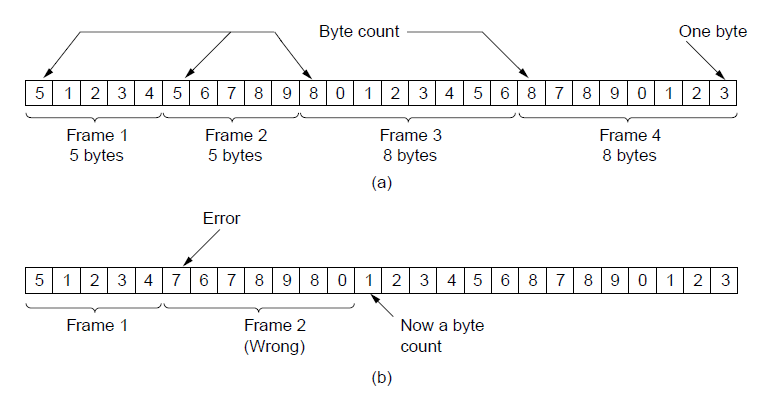
\includegraphics[width=10cm, height=5cm]{brojanjeBajtova}\\
\end{center}
\subsection{Umetanje bajtova}
Kada počinje novi okvir, ubaciću specijalnu sekvencu koja označava početak okvira. Kada primalac vidi tu spec. sekvencu, zna da je to početak okvira. Bolje je ideja od prethodne jer omogućava lakši oporavak od greške. Ako postoji greška u tom okviru, neće se propagirati na dalje okvire jer će naići nova sekvenca koja pokazuje da je tu početak novog okvira. U nekom momentu, za taj okvir u kome postoji greška, detekcija grešaka će shvatiti da tu postoji greška i ponove će zahtevati slanje okvira. Ako se desi da je greška baš na toj spec. sekvenci, onda će primalac uzeti dva okvira kao jedan okvir.  \\

Postoji jedan problem. Šta ako je ta spec. sekvenca, tj. indikator, unutar podatka?\\
Rešenje: Pre nego što pošiljalac pošalje okvir, on prođe kroz sadržaj i kod svih indikatora unutar podataka (koji odgovaraju toj specijalnoj sekvenci, tj. indikatoru koji nama služi za početak okvira, a to može biti neki specijalan bajt) umetne ESC sekvencu. Primalac čita podatke i naleti na taj indikator, ako pre njega nije naišao na ESC, to znači da je stvarno početak paketa. Ako naleti na indikator, a pre njega je bio ESC, to znači da to nije indikator početka okvira, nego je stvarno podatak. \\

Šta ako je poslednja informacija bude ESC? Onda će ići ESC pa indikator, što znači da će primalac, dok čita to , promašiti početak novog okvira. Rešenje je da pošiljalac kada šalje podataka eskejpuje sve indikatore i sve ESC koji su podaci. Primalac, kad dobije informaciju, skida esc i onda zna da je to bio pravi ESC ili ESC koji je umetnut. Primalac uvek skida prvi eskejp i zadržava naredni podatak. 
\begin{center}
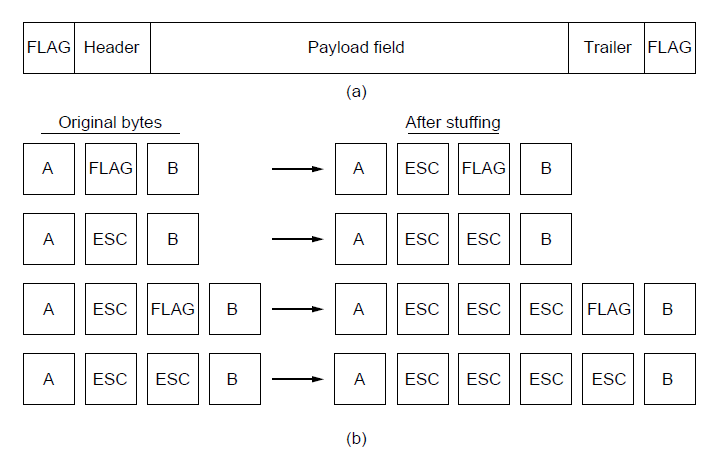
\includegraphics[width=10cm, height=6cm]{umetanjeBajtova}\\
\end{center}
\subsection{Umetanje bitova}
Slična ideja, samo sad ne vršimo parsiranje bajt po bajt, nego bit po bit. Praksa je da se koristi identifikator 6 uzastopnih jedinica. One predstavljaju početak okvira.\\

Šta ako se u okviru podataka desi da se nađu 6 uzastopnih jedinica? Pošiljalac treba da se pobrine da u okviru podataka ne postoji nigde 6 uzastopnih jedinica. Kako postiže to? Prilikom slanja prolazi kroz podatke i ako postoji negde ta sekvenca jedinica, on umeće nulu posle pete jedinice. Primalac kada vidi 6 jedinica, zna da tu počinje okvir, a kada naiđe na 5 jedinica gde je sledeća nula, on zna da je ta nula umetnuta tu, skida je i ne posmatra je kao podatak.\\

Sledeći korak je detekcija i korekcija grešaka. Sada znamo gde su granice okvira, a može da se desi da se desilo promena jednog bita baš u sekvenci 6 jedinica, što znači da je primalac uzeo kao jedan okvir dva prava okvira. Mehanizam za detekciju grešaka može da shvati da se tu pojavila greška. Traži ponovno slanje njih. Gde god da se desi greška, sloj veze treba da bude dovoljno otporan na nju.
\begin{center}
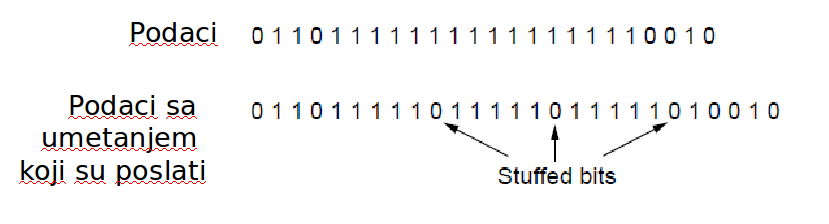
\includegraphics[width=10cm, height=3cm]{umetanjeBitova}\\
\end{center}
\section{Kodiranje grešaka u sloju veze}
(preuzeto iz beleški sa predavanja)\\

Dolazi do greške na nekim bitovima zbog šuma ili zbog prekida rada (ne zanima nas uzrok greške). Greška može da se desi sa nekom šansom (da ima verovatnoću), ali može da ima i različite distribucije pojavljivanja. Znači, treba da imamo u vidu tip greške: 
\begin{itemize}
  \item \textbf{ravnomerna}  - npr. jedna na svakih hiljadu bitova(ako govorimo o verovatnoći 0.001), nastaje zbog šuma
  \item \textbf{rafalna} - javlja se na velikom broju uzastopnih bitova, npr. zbog varničenja, signal se potupuno naruši
\end{itemize} 
Šta možemo da uradimo? Možemo detekciju grešaka sa retransmisijom (ponovno slanje) a može da se uradi i korekcija grešaka (podatak nosi sa sobom dovoljno informacija da se ispravi greška i ne zahteva ponovno slanje).\\
Pristup dodavanje redudantnosti:
\begin{itemize}
  \item \textbf{detekcija grešaka}  - dodavanje kontrolnih bitova\\
  Naivni pristup podrazumeva da pri slanju svakog okvira šaljemo i njegovu kopiju. Kopija služi za detekciju grešaka. Moć detekcije je jako dobra, detektuje se veliki broj grešaka, ali je loše jer se mnogo podataka koristi samo za detekciju grešaka. Može da se desi greška baš u istom bitu i originala i kopije. Ali, cilj detekcije grešaka je da se razreši što više grešaka (fokus je na onim greškama nastalim kao posledica šuma), a da se pritom koristi što manje bitova.
  \item \textbf{kodovi za korekciju grešaka} - dodavanje još bitova koje omugućavaju korekciju\\
  ------------------------dopuni----------------------\\
  Kodna reč se sastoji od $D$ bitova podataka i $R$ kontrolnih bitova. Pošiljalac izračuna $R$ kontrolnih bitova kao funkciju od $D$ i potom šalje svih $D+R$ bitova. Primalac prihvata $D+R$ sa potencijalnim greškama na bilo kom od bitova. Računa $R_{2}$ kontrolnih bitova na osnovu $D$ po istom algoritmu kao pošiljalac. Greška se javila ukoliko $R$ nije isto kao $R_{2}$.\\
  ----------------------------------------------\\
  Intuicija iza kodova za greške?\\
  Imamo mnogo manji skup validnih kodnih reči u odnosu na skup svih mogućih reči. Ukoliko imamo N bitova, onda imamo $2^{N}$ mogućih reči. Ako $R < N$ bitova (predstavljaju bitove za grešku), onda je skup validnih reči $2^{N-R} $. Kada pošiljalac pošalje validnu kodnu reč koliko je šansa da, ako je došlo do greške, to opet bude validna reč? Slučajno odabrana reč ima malu šansu da bude i validna $ \Rightarrow $ mala šansa da će se desiti greška i da će nakon toga reč i dalje biti validna. Nadudavanjem prostora redudantnih reči smanjujemo verovatnoću za nastajanje greške.
\end{itemize} 
\subsection{Hamingovo rastojanje}
\textit{Hamingovo rastojanje} je minimalan broj inverzija bitova potrebnih da se od jedne reči dobije neka druga reč. \\
\textit{Hamingovo rastojanje koda} je minimalno Hamingovo rastojanje između svih parova validnih kodnih reči.\\
Ukoliko imamo validne reči:
\begin{center}
111000\\
111111\\
000000\\
000111
\end{center}
shvatamo da imamo $ 2^{6} $ mogućih reči, od kojih su samo 4 validne. To znači da ako želim da šaljem poruke, jedine poruke koje mogu da pošaljem su ove 4 reči. Prva može da predstavi 0, druga može 1, itd. To znači da se preslikavaju skupovi bitova u neku vrednost. Na drugoj strani znamo skup validnih reči, tako da možemo da detektujemo grešku. \\

Šta je najveća greška koju možemo da detektujemo?\\
Hamingovo rastojanje ovih validnih reči je 3 (mora da se napravi minimum 3 inverzije da bi se iz jedne reči prešlo u drugu).
Na primer, ako se u reči 111000 desi na dva bita greška, pa dobijemo recimo reč 101010, možemo da utvrdimo da ova reč nije validna. Ali ako se, na primer, za reč 000111 desi trobitna greška, pa dobijemo reč 000000, onda ne možemo da utvrdimo da je došlo do greške. $ \Rightarrow $ za trobitne greške ne možemo da detektujemo grešku.\\
\textbf{Da bi se pouzdano otkrilo do $d$ grešaka, Hamingovo rastojanje koda mora biti najmanje $d+1$!}. Drugi način definisanja: ako je H.r. $d$ onda možemo da detektujemo $d-1$bitnu grešku.\\
Ovo nije efikasan algoritam, ali je teorijski dobar. Ima veliku redudantnost, tj. koristili smo 6 bitova da predstavimo samo 4 vrednosti. Primalac mora da prolazi kroz ceo spisak validnih reči kada čita podatke, što nije efikasno.\\

Kolika je najveća greška koja se može korektovati?\\
Ako se pri greški pojavi reč koja je susedna nekoj validnoj reči, ja verovatno mogu da pretpostavim, za Ham. rast. 3, da mogu da ispravim jednobitnu grešku. Samo nađem najbližu susednu validnu reč i našli smo korekciju. Ako se naiđe na reč iz većeg susedstva, odnosno greška veća od jednog  bita, onda ne mogu da odradim korekciju. \\
\textbf{Za kod sa Hamingovim rastojanjem $2d+1$ najviše $d$ grešaka se uvek može ispraviti do najbliže ispravne validne reči.} Drugi način definisanja: ako je H.r. $d$, onda najveća greška koja može da se ispravi je $\lfloor d/2 \rfloor$.

\section{Detekcija grešaka u sloju veze}
(preuzeto iz beleški sa predavanja)\\

Detekcija omogućava samo indirektnu  popravku jer zahteva retransmisiju. Koristimo tri algoritma u praksi:
\begin{itemize}
  \item Provera parnosti
  \item Kontrolni zbirovi
  \item Ciklične provere redudanse CRC
\end{itemize}
\subsection{Provera parnosti}
Retko se koristi jer ima slabu moć, odnosno samo za jednobitne greške radi.\\
Za D bitova podataka, dodamo jedan kontrolni bit koji predstavlja sumu bitova podataka. Suma je bez prenosa, odnosno suma po modulu 2. Moć ove tehnike je uslovljena Hamingovim rastojanjem. \\
Ako imamo podatak 0101, dodajemo 0 na kraj kao kontrolni bit za proveru parnosti. Skup validnih reči je $ 2^{4} $. Hamingovo rastojanje je 2 (mora da se menja i bit za proveru parnosti), pa je moć detekcije jedan. \\
 Problem je što loše radi za rafalne greške. Postoji 50\% šanse da se sa ovim algoritmom detektuje dvobitna ili višebitna greška.
 
\subsection{Kontrolni zbirovi}
Koriste se za rafalne greške. Problem kod rafalnih grešaka je što se one dešavaju uzastopno.\\
Opšti pristup:\\
Možemo da preuredimo naše bitove. Ne posmatramo bit po bit, nego imamo bafer gde možemo da prepakujemo bitove po kolonama i posle N bitova stavimo novu kolonu. Time dobijamo da se rafalne greške preraspodele u posebne kolone i onda radimo provere parnosti po redovima. Susedni bitovi se premeštaju u različite redove, pa je mala šansa da se u istom redu nađu greške koje su bile jedne pored druge. Što je širi registar, manja je šansa da će rafalna greška biti u istom redu i manja šansa da će se greška desiti.(?? dopuni, proveri ispravnost gde se koristi red, gde kolona, nešto je mešao to na predavanjima)
\subsubsection{Internet kontrolni zbir}
Konkretna implementacija prethodnog opšteg pristupa. Računa se u aritmetici nepotpunog komplimenta. Postoje dve reprezentacije nule. Jedna nula može da se iskoristi da predstavi da kontrolni zbir ne postoji, tj. inicijalno zbir koji dodajemo je nula i dodajemo mu prenos sa pozicije najveće težine. Kontrolni zbir ima 16 bitova i predstavlja nepotpuni komplement sume reči po kolonama.\\
Proces slanja:\\
\begin{enumerate}
\item složiti podatke kao šesnaestobitne reči jednu ispod druge
\item postaviti nule na pozicije kontrolnog zbira
\item eventualni prenos sa pozicije najviše težine  se prenosi na početak (to je sabiranje u nepotpunom komplementu)
\item negiramo dobijenu sumu i time dobijemo kontrolni zbir
\begin{center}
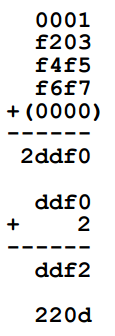
\includegraphics[width=2cm, height=5cm]{kontZbir}\\
\end{center}
\end{enumerate}
Proces prihvatanja:
\begin{enumerate}
\item složiti podatke kao šesnaestobitne reči jednu ispod druge, uključujući i reč za kontrolni zbir
\item ako postoji prenos sa pozicije najviše težine, dodamo ga na najniži bit
\item  negiramo rezultat i proverimo da li je nule; ako jeste, onda je sve u redu
\begin{center}
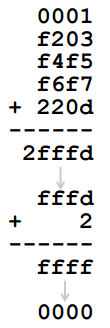
\includegraphics[width=2cm, height=5cm]{kontZbir2}\\
\end{center}
\end{enumerate}
Kontrolni zbir se koristi i na višim slojevima, ne samo na sloju veze.
\subsection{CRC}
Koristi se i za ravnomerne i za rafalne greške. Ima mali broj dodatnih bitova, a detektuje i četvorobitne greške. Još bolja detekcija od prethodnih pristupa. \\
Sekvenca bitova se smatra polinomom čiji su koeficijenti samo nule i jedinice. Tamo gde je jedan, to znači da u polinomu postoji taj stepen, ako je nula, znaci da ne postoji.\\
Cilj je da se napravi neki drugi polinom na osnovu polinoma koji želimo da pošaljemo i taj konačni polinom koji treba da se pošalje (sastoji se od početnog polinoma i tog napravljenog polinoma) treba da bude deljiv sa nekim drugim unapred određenim polinomom koji se naziva \textit{generator} i kojeg znaju i primalac i pošiljalac. Za datih n bitova podataka, generišemo k kontrolnih bitova (određuje se preko toga koliki je najveći mogući ostatak koji može da se dobije deljenjem sa generatorom) tako da n+k bitova bude deljivo sa generatorom C.\\
Postupak slanja: 
\begin{enumerate}
\item proširiti n bitova sa k nula
\item podeliti broj sa odabranim brojem C
\item zadržimo samo ostatak 
\item dodamo ostatak na prosiren broj
\end{enumerate}
Primanje podataka:
\begin{enumerate}
\item podeliti poruku sa brojem C i proveriti da li je ostatak pri deljenju jednak nuli
\end{enumerate}
Primer: želimo da pošaljemo niz bitova 1101011111 (polinom $ x^{9}+x^{8}+x^{6}+x^{4}+x^{3}+x^{2}+x^{1}+1 $, dalje radimo sa binarnim vrednostima i aritmetikom po modulu 2, ignorišemo potencijalne prenose sa najviše pozicije). Imamo delilac $C(x)= x^{4} + x^{1} + 1 $, što znači da je C=10011 i k=4.
\begin{center}
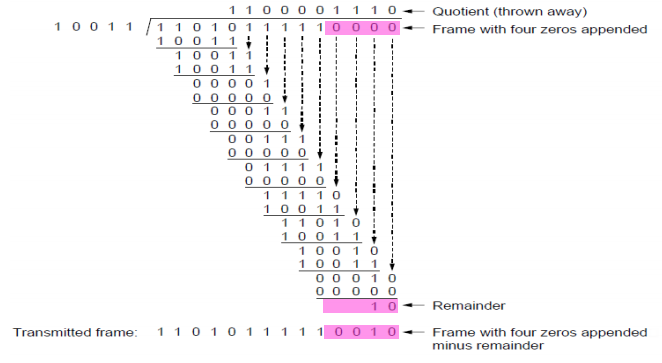
\includegraphics[width=12cm, height=7cm]{crc}\\
\end{center}
CRC detekcija se radi i na višim slojevima, ne samo na sloju veze.

\section{Korekcija grešaka u sloju veze}
(preuzeto iz beleški sa predavanja)\\

Moguće je konstruisati kodove koji su  u stanju i da poprave grešku. Jedni od takvih su Hamingovi kodovi za korekciju koji imaju Ham. rastojanje koda 3. \\
Šta će nam korekcija, ako možemo da detektujemo i uradimo retransmisiju? Postoje situacije kad nam je bolje jedno, a kad drugo. Odlučivanje o tome šta ćemo koristiti je bazirano na nekim parametrima. Jedan od tih parametara je način dešavanje greške, tj. distribucija greške.\\
 Ako se dešavaju rafalne greške, nepredviđene, bolje je koristiti detekciju sa retransmisijom jer se greška javlja npr. jednom u 100 paketa, a za detekciju je potrebno manje bitova nego za korekciju (ako bismo koristili korekciju, to znači da bismo za svakih 100 paketa uvek slali više podataka nego što je potrebno za detekciju). Znači detekcija se koristi \textit{kad su greške neočekivane, tj. retke i rafalne, a kad se dese, onda nema veze i ako su velike}.Najčešće se koristi u sloju veze u kombinacijisa retransmisijom okvira.\\
 Ako imamo neki šum koji se stalno javlja, loše je raditi detekciju sa retransmisijom jer postoji mogućnost da ćemo za svaki paket da radimo retransmisiju i zato koristimo korekciju. Znači, korekcija se koristi \textit{kad su greške očekivane, tj. šum se javio ili kada nema vremena za retransmisiju} i najčešće se radi na fizičkom sloju.\\\\

Intuicija iza kodova za korekciju grešaka objašnjena u nekom od prethodnih pitanja.\\

\textbf{Hamingov kod za korekciju:}\\

Ideja je da se kontrolni bitovi stavljaju na pozicije koje predstavljaju stepene dvojke, a na preostalim mestima upisujem bitove za podatke. Kontrolni bitovi služe da napumpaju prostor redudantnosti. Koriste se n bitova podataka i k kontrolnih bitova gde važi $n = 2^{k}-k-1$ (npr. n=4, k=3). Kontrolni bit na poziciji \textit{i} se dalje računa kao bit parnosti za bitove čije pozicije u binarnoj reprezentaciji imaju 1 na \textit{i}-tom mestu. Npr. ako imamo 7 pozicija, 4 za podatke (neka je podatak npr. 0101), 3 za kontrolne bitove (pozicije 1,2,4), onda bit 1 pokriva pozicije 1,3,5,7 (1=0001,3=0011...to su pozicije koje imaju 1 u svom binarnom zapisu), bit 2 pokriva poziije 2,3,6,7 (2=0010, 3=0011,..), a bit 4 pokriva pozicije 4,5,6,7 (4=0100, 5=0101, …). Dobijamo:
\begin{center}
	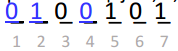
\includegraphics[scale=0.5]{korek}
\end{center}
gde se kontrolni bit na poziciji 1 računa kao $ p_{1} = 0+1+1 = 0$ što su vrednosti na pozicijama 3,5,7 bez pozicije 1, jer za poziciju jedan računamo kontrolni bit. Dalje imamo: $ p_{2} = 0+0+1 = 1$ i $ p_{4} = 1+0+1 = 0$. Ovakav niz od 7 bitova se šalje.\\

Kada primalac primi ovaj niz bitova, on ponavlja isti proces. Ponovo računa kontrolne bitove tako što sabira odgovarajuće pozicije. Pretpostavimo da je stigla poruka sa greškom, 0100111. Primalac racuna kontrolni bit kao zbir bitova na pozicijama 1,3,5,7. $ p_{1} = 0+0+1+1 = 0$. Isto radi i za kontr. bit $ p_{2} = 1+0+1+1 = 1$ (odmah signalizira da je doslo do greške, čim se nije dobila nula). Računa i $ p_{4} = 0+1+1+1 = 1$. Nakon ovoga složi dobijene kontrolne bitove kao binarni broj i dobije \textit{sindrom} (u ovom slučaju je to 110) koji otkriva na kojoj poziciji je došlo do greške. Korekcija će se izvršiti komplementiranjem bita na toj poziciji. Kada je sindrom jednak nuli, onda nema greške.\\

Ovaj algoritam se obično ne koristi u praksi, već neki mnogo složeniji algoritmi kao što su:
\begin{itemize}
  \item Konvolucioni kodovi (omogućavaju korekciju grešaka za k bitova odjednom)
  \item Rid-Solomonovi kodovi
  \item Metoda parnosti za malu gustinu (LDPC-low density parity check) 
\end{itemize}
\section{Sloj veze, tipovi servisa, okruženje, utopijski jednosmerni protokol}
(preuzeto iz beleški sa časa)\\

\subsection{Tipovi servisa}

\begin{enumerate}
  \item \textbf{Servis bez uspostave veze i bez potvrde prijema}\\
  Šalju se okviri bilo kojim redosledom, na drugu stranu ne moraju da stižu u redosledu u kojem smo slali. Nemamo mehanizam da utvrdimo da li je stiglo, ako se desi greška, ispraviće se u višem sloju, neće se vršti retransmisija, tj. pouzdanost se odlaže višim nivoima jer se retko dešavaju greške. Ovo se radi zbog brzine. Primer je Eternet.
  \item \textbf{Servis bez uspostave veze i sa potvrdom prijema}\\
  Za svaki okvir dobijemo sa druge strane potvrdu da je stigao, ako nije validan, ne dobijemo potvrdu. Ako ne stigne potvrda, radi se retransmisija. Primer je WiFi.
  \item \textbf{Servis sa uspostavom veze i sa potvrdom prijema}\\
  Uspostava veze omogućava da podaci teku istim redom kojim su i poslati. (primalac prima podatke u istom redosledu u kojem su i poslati). Retko se koristi.
\end{enumerate}

\subsection{Okruženje}
Sloj veze je obično realizovan delom na mrežnoj kartici, a drugim delom na nivou operativnog sistema. 
\begin{center}
	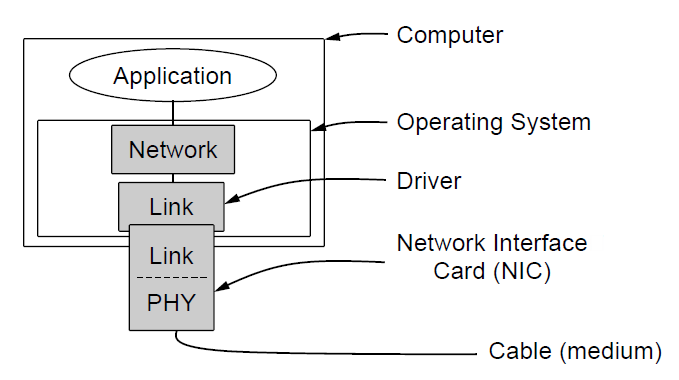
\includegraphics[scale=0.3]{okruzenjeSV}
\end{center}
Komunikacija sloja veze sa ostalim slojevima:
\begin{itemize}
  \item prema mrežnom sloju\\
  Sloj veze dobija od mrežnog sloja sledeći paket, ne može da zahteva neki određen paket i ne može da puta da se traži isti paket. Mora da se obezbede informacije ako se izgube, tj. informacije baferiše pošiljalac.\\
  Kada šaljemo mrežnom sloju paket, samo jednom smemo da šaljemo jedan paket, ne može dva puta da se šalje ako smo pogrešili.
  \item prema fizičkom sloju\\
  Od fizičkog sloja zahtevamo samo jednom jedan okvir. Šaljemo fizičkom sloju samo jednom paket. 
\end{itemize}

Postoje i neki događaji i tajmeri definisani na sloju veze:
\begin{itemize}
  \item wait\textunderscore for\textunderscore event(\&event) - blokirajuća funkcija sve dok se ne dogodi neki event. Čeka na paket/okvir/istek tajmera.
  \item start\textunderscore timer(seq\textunderscore nr) - pokreće tajmer
  \item stop\textunderscore timer(seq\textunderscore nr) - prekida tajmer
  \item start\textunderscore ack\textunderscore timer() - pokreće tajmer za okvir potvrde ACK
  \item stop\textunderscore ack\textunderscore timer() - prekida tajmer za okvir potvrde ACK
\end{itemize}

Protokoli na sloju veze su u\textbf{topijski jednosmerni protokol, „stani i čekaj“ protokol za kanal bez grešaka, „stani i čekaj“ protokol za kanal sa greškama}.
\subsection{Utopijski jednosmerni protokol}
Ovaj protokol ne predviđa pojavu greške, pretpostavlja da su primalac i pošiljalac iste brzine i prenos podataka je jednosmeran.\\

Pošiljalac u beskonačnoj petlji uzima od mrežnog sloja paket po paket i stvara okvir i prosleđuje to fizičkom sloju. Nema mogućnost istovremenog slanja podataka.\\
Primalac u beskonačnoj petlji čeka na događaj. Kad mu stigne događaj (stigao novi okvir) blokirajuća komanda se odblokira. Pretpostavlja se da je okvir validan. Primalac tad iz fizičkog okvira učita okvir i prosledi dalje mrežnom sloju. 
\begin{center}
	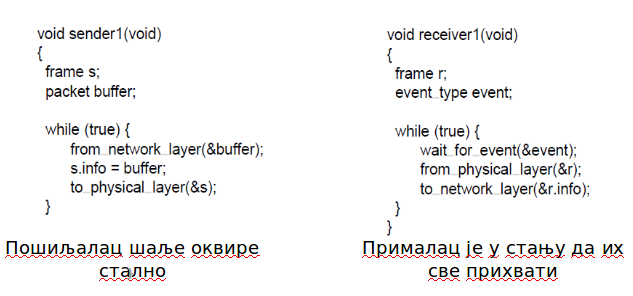
\includegraphics[scale=0.5]{utopijski}
\end{center}
\section{Kontrola toka, ARQ, pauze (tajmauti), duplikati, protokol „stani i čekaj“ za savršen i nesavršen kanal}
(preuzeto iz beleški sa vežbi)\\

Šta ako pošiljalac i primalac nemaju iste brzine slanja, odnosno primanja? Potrebna je kontrola toka.
Kontrola toka je sinhronizacija komunikacije između pošiljaoca i primaoca. Primalac ne sme da bude zatrpan od strane pošiljaoca.\\
\begin{center}
	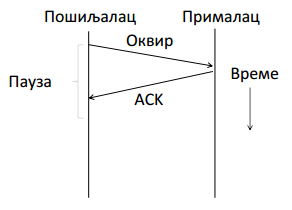
\includegraphics[scale=0.5]{razlBrzine}
\end{center}

\subsection{Protokol „stani i čekaj“ za savršen kanal}
Pretpostavljamo da je kanal savršen, tj. nema grešaka niti izgubljenih okvira i ovaj protokol garantuje usaglašenost u brzini komunikacije. \\
Pošiljalac šalje okvir i čeka potvrdu da je primljen okvir sa druge strane. Ta potvrda znači da je primalac spreman dalje da prima podatke. Primalac kao potrvdu šalje prazan okvir - ack. Šalje se okvir po okvir, što je vrlo neefikasno.
\begin{center}
	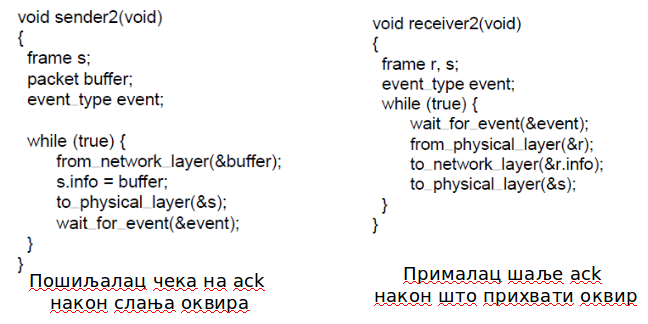
\includegraphics[scale=0.5]{staniIcekaj1}
\end{center}

\subsection{ARQ - Automatic Repeat reQuest}
Šta se dešava ako je nesavršen kanal? Može da se desi da okvir nije stigao na drugu stranu ili da je okvir stigao, ali nije validan i može da se desi da okvir stigne uspešno, ali da se potvrda izgubi. U tom slučaju se radi detekcija i retransmisija ARQ ili korekcija grešaka (obrađeno, više se tiče fizičkog sloja). 
\\
ARQ se obično koristi kada su greške uobičajene i kada se moraju ispraviti, npr. kod WiFi i TCP.\\
Osnovna ideja je da primalac šalje potvrdu o prijemu ispravnog okvira ACK (to je takođe okvir), a pošiljalac uključuje tajmer čim pošalje okvir i automatski šalje ponovo okvir ako istekne vremenska pauza (timeout), osim ako u međuvremenu nije pristigao ACK.
Na sledećoj slici je prikazan scenario sa gubitkom i retransmisijom.
\begin{center}
	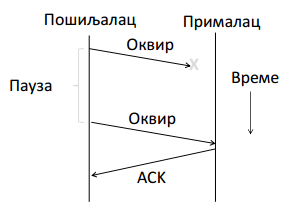
\includegraphics[scale=0.5]{ARQ1}
\end{center}
Osnovni cilj je da okviri budu ispravni i da se ne dupliraju, a sekundarni cilj je da komunikacija bude efikasna.\\

Postavljaju se dva ključna pitanja:
\begin{enumerate}
	\item \textbf{Kolika treba da bude pauza, tj. vreme za koje timeout ističe?}\\
	Pauza ne treba da bude prevelika jer će primalac previše da čeka izgubljene pakete i doći će do neiskorišćenosti kanala. Ne treba da bude ni premala da se ne bi stalno radila retransmisija, odnosno, stalno prekidamo primaoca kada želi da pošalje potvrdu. Dužinu pauze je jednostavno odrediti za LAN (jasna je gornja granica, malo odstupanje), ali je teško za Internet (veliko odstupanje, nema jasne gornje granice).
	\item \textbf{Kako da se izbegne interpretiranje dupliranih okvira kao novih?}\\
	Situacija kada se ACK izgubi dovodi do toga da je moguće interpretirati dupliran okvir kao novi poslati okvir.
\begin{center}
	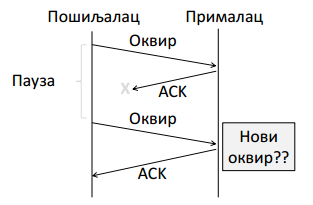
\includegraphics[scale=0.5]{ARQ2}
\end{center}
	Situacija kada je prekratka pauza može da dovede do iste situacije.
\begin{center}
	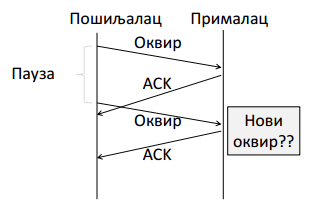
\includegraphics[scale=0.5]{ARQ3}
\end{center}
Iz ovoga izvlačimo da je neophodno da okviri i ACK-ovi nose sa sobom nekakvu oznaku da bi se izbegli duplikati. Dovoljno je da se razlikuje samo trenutni okvir od narednog okvira, što se može predstaviti jednim bitom.
(radi se nekakvo invertovanje bitova, prvi put kad se šalje okvir bit je 0...??)
\end{enumerate}
\subsection{Protokol „stani i čekaj“ za nesavršen kanal}
\begin{center}
	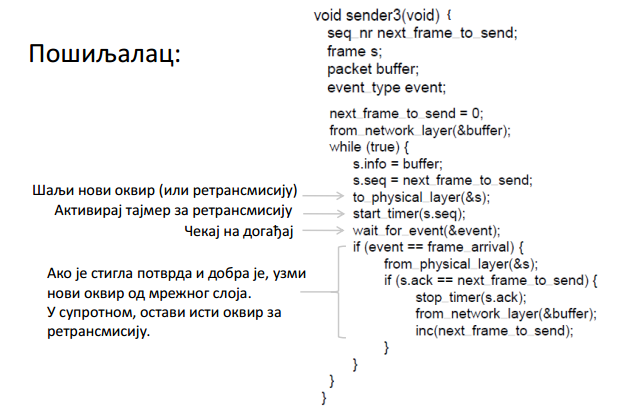
\includegraphics[scale=0.5]{staniIcekaj2}
	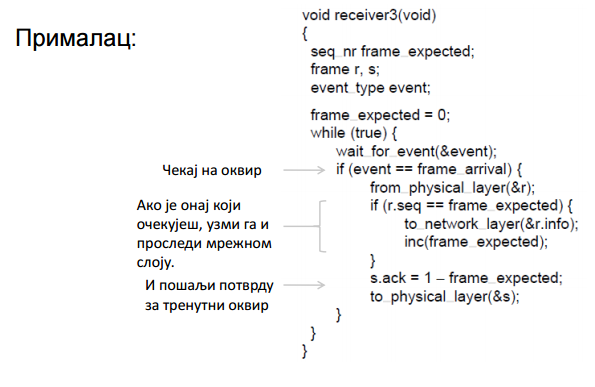
\includegraphics[scale=0.5]{staniIcekaj3}
\end{center}
Ograničenja ovog protokola: 
\begin{itemize}
  \item \textbf{neefikasan}\\
  U datom momentu samo 1 paket prolazi kroz komunikacioni kanal. Prihvatljivo je za LAN, ali vrlo neefikasno za visok BDP. Primer: $B = 1 Mb/s$ $ D=50ms $. Proveriti koliko okvira u sekundi se prenese, i koliko okvira   u sekundi ako je $B = 10 Mb/s$.
\end{itemize}
\section{Protokol kliznih prozora u sloju veze, „1-bitni“, „vrati se N“, „selektivno ponavljanje“}

\subsection{Protokol kliznih prozora u sloju veze}

Uop\v{s}tenje protokola "stani i \v{c}ekaj". Omogu\'{c}ava da u svakom momentu W okvira bude u kanalu. W okvira za RTT (\textit{round trip time} - vreme potrebno da okvir ode i da stigne potvrda za njega).\\
Svakom okviru se dodeljuje redni broj, na osnovu kog se identifikuje. Po\v{s}iljalac i primalac imaju opseg u okviru kog primaju okvire.\\
Po\v{s}iljac ima na raspolaganju W okvira koje mo\v{z}e da po\v{s}alje. Mora da ih baferuje zbog eventualne retransmisije. Sa pristiglim \textit{ack}-ovima po\v{s}iljalac pomera prozor.\\
Primalac ima na raspolaganju prostor za nekoliko okvira koje mo\v{z}e da prihvati. Mora da poseduje bafer za njih. Kako sti\v{z}u novi okviri prozor se pomera.\\
\begin{center}
	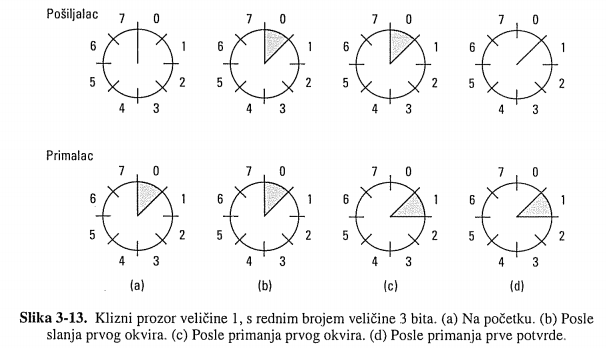
\includegraphics[scale=0.5]{klizni_prozor}
\end{center}
Ve\'{c}i prozori omogu\'{c}avaju proto\v{c}nu odbranu za efikasniju upotrebu kanala. Stani i \v{c}ekaj (W=1) je neefikasan, posebno za du\v{z}e kanale (po\v{s}iljalac \v{s}alje okvir i \v{c}eka potvrdu o prijemu). \v{Z}elim da va\v{z}i $ W \geq{} 2BD + 1 $ u cilju \v{s}to boljeg iskori\v{s}\'{c}enja.

\subsection{"1-bitni"}

Protokol kliznih prozora maksimalne veli\v{c}ine 1. Nema odvojenih algoritama za po\v{s}iljaoca i primaoca, jer sada i jedan i drugi mogu da \v{s}alju i primaju. Za \textit{ack} koristimo okvir iz suprotnog pravca ("\v{s}lepanje").

\begin{center}
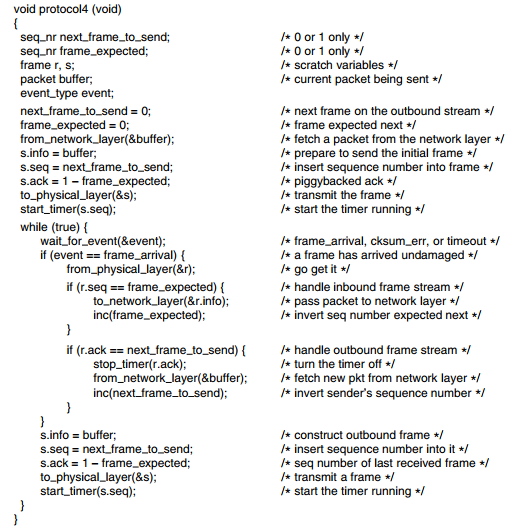
\includegraphics[scale=0.7]{1-bitni-kod}
\end{center}
Ovaj algoritam radi korektno, ali mo\v{z}e do\'{c}i do usporenja ukoliko istovremeno zapo\v{c}nu slanje, jer \'{c}e tako biti izostavljen \textit{ack}, te \'{c}e biti ponovljenih slanja.

\subsection{"Vrati se N"}

Primalac prihvata samo okvire koji sti\v{z}u redom, odbacuje sve koji uslede nakon spornog (okvira koji nije primljen ispravno). Nakon \v{s}to tajmoutuje, ponavljaju se svi nepotvr\dj{}eni okviri do kraja prozora.

\begin{center}
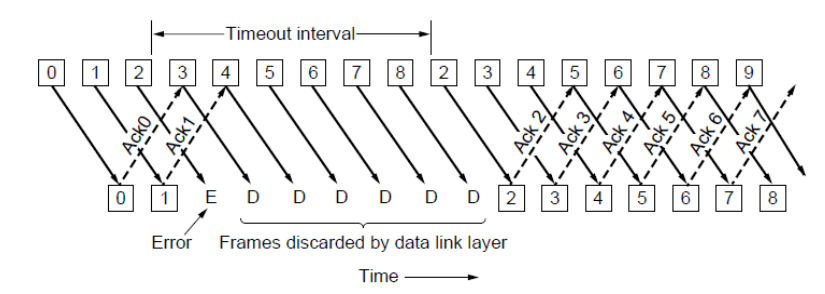
\includegraphics[scale=0.4]{vrati-n}
\end{center}
Jednostavan algoritam na strani primaoca, potreban mu je bafer za samo jedan okvir. Nepotrebno tro\v{s}enje protoka u slu\v{c}aju velikih prozora, u najgorem slu\v{c}aju je potrebno ponoviti slanje celog prozora.

\subsection{"Selektivno ponavljanje"}

Primalac prihvata okvir sve dok je redni broj okvira u opsegu definisanom kliznim prozorom. Negativni \textit{ack} informi\v{s}e po\v{s}iljaoca da ponovo po\v{s}alje problemati\v{c}ni okvir, pre isteka tajmauta za ceo prozor.

\begin{center}
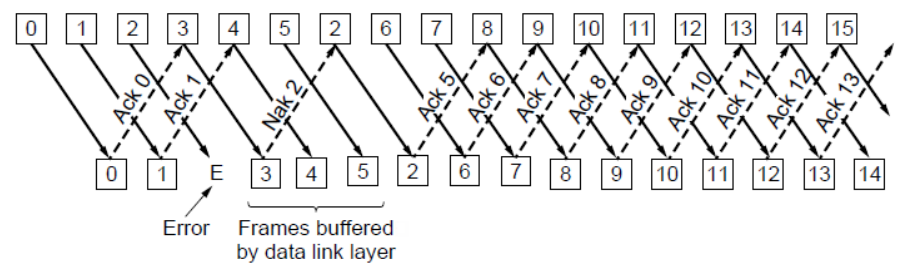
\includegraphics[scale=0.4]{selektivno-ponavljanje}
\end{center}
Slo\v{z}eniji je za implementaciju od "vrati se N" zbog baferisanja pri primanju i vi\v{s}estrukih tajmera pri slanju. Efikasnija upotreba protoka, jer se sada \v{s}alju ponovo samo izgubljeni okviri.\\
Opseg brojeva okvira mora biti barem dva puta ve\'{c}i od veli\v{c}ine prozora kako bi se izbegli problemi sa retransimisijom okvira.

\begin{center}
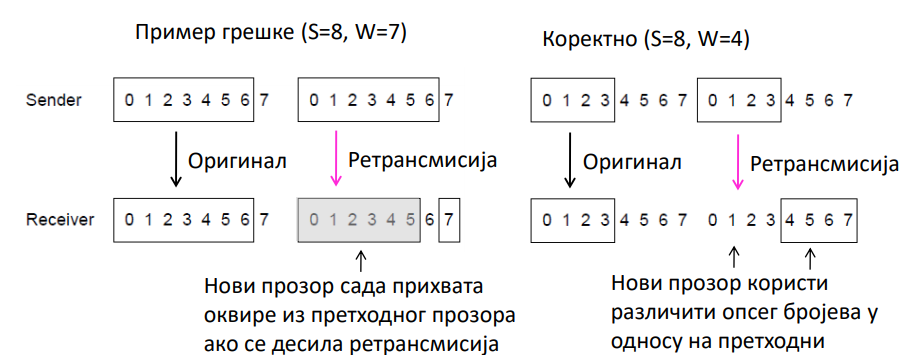
\includegraphics[scale=0.4]{selektivno-zahtevi}
\end{center}

U prvom slu\v{c}aju, primalac nakon prijema prvih 7 okvira, o\v{c}ekuje okvire 7, 0, 1, 2, 3, 4, i 5, \v{s}to je u konfliktu sa paketima koji su ve\'{c} primljeni. Ako bi po\v{s}iljalac iz nekog razloga ponovio slanje prethodnih paketa, oni bi ponovo bili pogre\v{s}no prihva\'{c}eni i prosle\dj{}eni mre\v{z}nom sloju. U drugom slu\v{c}aju se ovo ne mo\v{z}e desiti.

\section{MAC podsloj, uloga, alokacija kanala, ALOHA protokol}

\subsection{MAC podsloj, uloga}

U svakoj mre\v{z}i u kojoj se koristi neusmereno emitovanje, glavni problem je kako odrediti ko \'{c}e koristiti kanal u situaciji kada ima vi\v{s}e zahteva. Protokoli kojima se odre\dj{}uje slede\'{c}i korisnik takvog kanala pripadaju podsloju sloja veze podataka, poznatom kao podsloj za \textbf{upravljanje pristupom medijumima} (\textit{Medium Access Control, MAC}. Protokol MAC je posebno va\v{z}an za lokalne mre\v{z}e u kojima se za komuniciranje naj\v{c}e\v{s}\'{c}e koristi kanal sa slobodnim pristupanjem.

\subsection{Alokacija kanala}

\begin{enumerate}
	\item Stati\v{c}ko dodeljivanje kanala
	\item Dinami\v{c}ko dodeljivanje kanala
\end{enumerate}

\subsubsection{Stati\v{c}ko dodeljivanje kanala}

Klasi\v{c}an na\v{c}in dodeljivanja jedinstvenog kanala jednom od kandidata na njega je multipleksiranje podelom frekvencije (FDM). Ukoliko postoji $N$ potencijalnih korisnika, propusni opseg se deli na $N$ jednakih delova, po jedan za svakog korisnika. Tako se korisnici ne ometaju me\dj{}usobno. Kada je broj po\v{s}iljalaca veliki ili se stalno menja, tehnika FDM ne zadovoljava. Tako\dj{}e, ako u nekom trenutku \v{z}eli da komunicira manje od $N$ korisnika, veliki deo opsega ostaje neiskori\v{s}\'{c}en. Suprotno, ukoliko vi\v{s}e korisnika \v{z}eli da komunicira, neki od njih nece mo\'{c}i. Drugi metod, sa sli\v{c}nim karakteristikama je TDM (multipleksiranje podelom vremena).

\subsubsection{Dinami\v{c}ko dodeljivanje kanala}

Da bi se razumeo problem, potrebno je sagledati pet osnovnih pretpostavki:
\begin{enumerate}
	\item Model stanica - model sadr\v{z}i $N$ nezavisnih stanica;
	\item Pretpostavka o jedinstvenom kanalu - za sve komunikacije na raspolaganju je jedan kanal;
	\item Pretpostavka o sukobljavanju - ako se dva okvira istovremeno emituju, oni se vremenski preklapaju \v{s}to rezultuje izobli\v{c}enim signalom. Ovaj doga\dj{}aj naziva se \textbf{sukobljavanje};
	\item Vremenski tok:
	\begin{itemize}
		\item Neprekidan vremenski tok - paket se mo\v{z}e poslati u bilo kom trenutku;
		\item Raspore\dj{}eno vreme - vreme podeljeno u intervale odre\dj{}ene veli\v{c}ine, slanje se podudara sa po\v{c}etkom intervala;
	\end{itemize}
	\item Pona\v{s}nje stanica:
	\begin{itemize}
		\item Oslu\v{s}kivanje saobra\'{c}aja na nosiocu podataka - pre upotrebe kanala, stanica mo\v{z}e proveriti da li je slobodan;
		\item Nema oslu\v{s}kivanja saobra\'{c}anja na nosiocu podataka - stanice ne proveravaju da li je kanal prazan, ve\'{c} odmah emituju okvire. Tek kasnije se utvr\dj{}uje da li je prenos uspe\v{s}an.
	\end{itemize}
\end{enumerate}
Za stavke 4 i 5 va\v{z}i jedna od dve postoje\'{c}e mogu\'{c}nosti.

\subsection{ALOHA protokol}

Nastao po ugledu na ra\v{c}unarsku mre\v{z}u koja je povezivala Havajska ostrva '60-ih godina. Postoje dve verzije sistema ALOHA:
\begin{itemize}
	\item \v{C}ista ALOHA
	\item Vremenski raspodeljena ALOHA
\end{itemize}
Kod ALOHA protokola se ne oslu\v{s}kuje saobra\'{c}aj pre slanja.

\subsubsection{\v{C}ista ALOHA}

Po\v{c}iva na jednostavnoj ideji, dozvoliti korisnicima da emituju uvek kada imaju podatke za slanje. Naravno, bi\'{c}e sukobljavanja, ali \'{c}e iz povratnih informacija po\v{s}iljalac jasno videti da je njegov okvir uni\v{s}ten. Kada utvrdi da je poslati okvir o\v{s}te\'{c}en, po\v{s}iljalac \'{c}e slu\v{c}ajno izabran period vremena sa\v{c}ekati eventualnu potvrdu prijema i nakon toga ponovo poslati okvir. Vreme \v{c}ekanja se bira nasumi\v{c}no kako bi se smanjila \v{s}ansa ponovnog sukoba istih paketa.

\begin{center}
	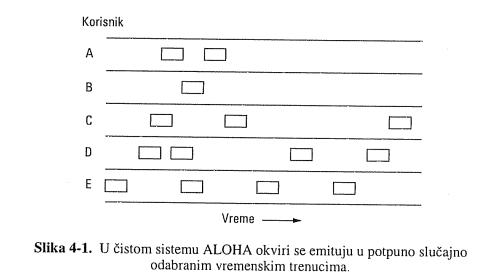
\includegraphics[scale=0.5]{aloha}
\end{center}

Osnovne karakteristike su mu jednostavnost i decentralizovanost. Ovaj algoritam se pokazuje kao prihvatljivo re\v{s}enje kada je malo optere\'{c}enje mre\v{z}e. Me\dj{}utim, algoritam ima lo\v{s}e karakteristike sa uve\'{c}anjem optere\'{c}enja mre\v{z}e. Eksperimentalno utvr\dj{}eno da 18\% okvira pro\dj{}e na drugu stranu.

\subsubsection{Vremenski raspore\dj{}ena ALOHA}

Kod vremenski raspodeljene neophodno je sinhronizovanje globalnog vremena. To se obi\v{c}no posti\v{z}e tako \v{s}to jedna stanica u predodre\dj{}enom intervalu \v{s}alje poseban signal. Time se vreme deli na intervale kona\v{c}ne du\v{z}ine. Emitovanje je dozvoljeno samo na po\v{c}etku intervala. Time se smanjuje verovatno\'{c}a da do\dj{}e do sukoba. Uspe\v{s}nost ovog algoritma je eksperimentalno utvr\dj{}ena i iznosi 36\%.

\section{CSMA, CSMA/CD, BEB}

Kako bi pobolj\v{s}ali karakteristike koje dobijamo sa ALOHA protokolima, koristimo \textbf{protokole za pristupanje uz oslu\v{s}kivanje saobra\'{c}aja na nosiocu podataka} (\textit{carrier sense protocols}). Oslu\v{s}kivanje saobra\'{c}aja ne garantuje da ne\'{c}e biti kolizija zbog ka\v{s}njenja signala.

\subsection{CSMA}

Kada stranica ima podatke za slanje, ona prvo oslu\v{s}ne kanal da bi utvrdila da li je zauzet. Ako na kanalu ima saobra\'{c}aja, stanica \v{c}eka, pa tek kada se kanal oslobodi \v{s}alje svoj okvir. Kada do\dj{}e do sukobljavanja, stranica \v{c}eka tokom nasumi\v{c}no odabranog perioda i po\v{c}inje ponovo. Postoji nekoliko varijacija CSMA protokola:
\begin{itemize}
	\item 1-trajni CSMA - nakon \v{s}to se kanal oslobodi, stanica \v{s}alje okvir sa verovatno\'{c}om jedan \v{c}im utvrdi da je kanal prazan
	\item Povremeni CSMA - kada utvrdi da je kanal zauzet, ne proverava svaki \v{c}as da li se oslobodio, ve\'{c} proverava nakon nasumi\v{c}no odabranog intervala
	\item p-trajni CSMA - ukoliko je kanal prazan, emituje se sa verovatno\'{c}om $p$, dok se sa verovatno\'{c}om $q=1-p$ odustaje od emitovanja do slede\'{c}eg vremenskog intervala
\end{itemize}

\begin{center}
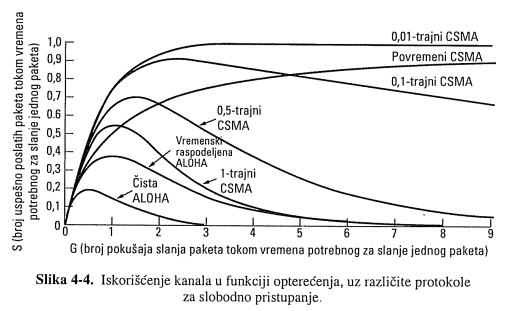
\includegraphics[scale=0.5]{csma}
\end{center}

\subsection{CSMA/CD}

Dodatno pobolj\v{s}anje predstavlja prekid emitovanja ukoliko stanica utvrdi da je do\v{s}lo do kolizije. Time bi se prekinulo ionako bespotrebno slanje izobli\v{c}enih podataka i u\v{s}tedelo vreme i propusni opseg. Ovakav protokol se naziva CSMA uz otkrivanje sukoba (\textit{CSMA with Collision Detection}). Minimalno vreme potrebno za otkrivanje sukoba jednako je vremenu putovanja od jedne stanice do druge, me\dj{}utim, mo\v{z}e se desiti, u najgorem slu\v{c}aju da to vreme bude dvostruko ve\'{c}e. U slu\v{c}aju da najudaljenija stanica po\v{c}ne sa emitovanjem ta\v{c}no u trenutku kad signal prve stigne do nje. U tom slu\v{c}aju \'{c}e informacija o sukobu sti\'{c}i do prve stanice mnogo kasnije. Zbog ovoga se \v{c}esto koristi ograni\v{c}enje za minimalnu du\v{z}inu poruke, kako bi se onemogu\'{c}ilo da stanica po\v{s}alje celu poruku pre nego \v{s}to uo\v{c}i koliziju.  Stanica koja \v{s}alje ne mo\v{z}e primati podatke jer se za oslu\v{s}kivanje kolizije koristi logika primaoca.

\subsection{BEB}

BEB (Binarno Eksponencijalno Odlaganje) protokoli su zapravo modifikacija p-trajnih CSMA protokola (\v{c}esto u kombinaciji sa detekcijom sukobljavanja). Naime, u slu\v{c}aju kolizije \v{c}eka se interval potreban da se po\v{s}alje 0 ili 1 okvir. Tada se ponovo poku\v{s}ava. Ukoliko se ponovo dogodi neuspeh, \v{c}eka se period vremena potreban da se po\v{s}alje izme\dj{}u 0 i 3 okvira. Pri svakom slede\'{c}em neuspehu interval se duplira. Ovako interval brzo raste, i dobija se velika efikasnost u prakti\v{c}noj primeni. Protokol CSMA/CD sa BEB je bio veoma kori\v{s}\'{c}en '80-ih i '90-ih za LAN mre\v{z}e.

\section{MAC protokoli zasnovani na redosledu, Token Ring}

Kako i CSMA daje relativno lo\v{s} rezultate pod visokim optere\'{c}enjem (visoki dodatni tro\v{s}kovi, vreme pristupa varira), potreban nam je protokol koji \'{c}e obezbediti prihvatljive performanse u uslovima visokog optere\'{c}enja.
MAC protokoli zasnovani na redosledu predstavljaju ure\dj{}ene protokole u kojima svaka stanica kada do\dj{}e na red mo\v{z}e da po\v{s}alje okvir ili da propust redosled, ukoliko nema potrebu da \v{s}alje. Ure\dj{}enje se mo\v{z}e definisati po tokenu koji se prosle\dj{}uje ili po vrednosti adrese.

\subsection{Token Ring}

\v{C}vorovi se organizuju u prsten. Token se prosle\dj{}uje u krug. Pravo slanja okvira ima samo \v{c}vor koji poseduje prsten.

\begin{center}
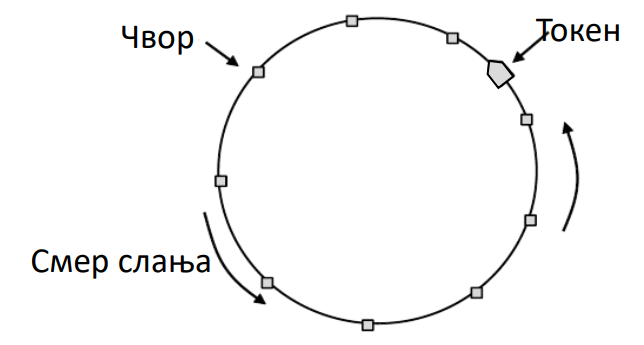
\includegraphics[scale=0.3]{token-ring}
\end{center}

Zajedno sa tokenom, i podaci idu samo u jednom smeru. Ta\v{c}nije, ukoliko stanica primi paket koji nije namenjen njoj, ona ga prosle\dj{}uje dalje u odgovaraju\'{c}em smeru. Ovde treba obezbediti da se paket ne vrti beskona\v{c}no kroz prsten. Uklanjanje paketa iz mre\v{z}e mo\v{z}e obaviti stanica kojoj je paket namenjen ili stanica koja je paket poslala (ukoliko paket obi\dj{}e ceo krug bez da na\dj{}e primaoca).

\subsection{Prednosti i mane}

Kako su svi tro\v{s}kovi unapred predefinisani i onemogu\'{c}ena kolizija, dobijamo efikasniji rad pri visokim optere\'{c}enjima. Tako\dj{}e, garantovano je da \'{c}e u razumnom roku svi (unapred definisanom) svaki \v{c}vor dobiti priliku da po\v{s}alje svoj okvir. Me\dj{}utim, i u ovom protokolu postoje nedostaci. Pre svega, tu je veliki tro\v{s}ak pri malim optere\'{c}enjima. Tako\dj{}e, mo\v{z}e se desiti da se u komunikaciji izgubi token. Ovi protokoli se primenjuju eksperimentalno, kao mogu\'{c}nost pobolj\v{s}anja. Me\dj{}utim, protokoli sa slu\v{c}ajno\v{s}\'{c}u se uglavnom mnogo bolje pokazuju i te\v{s}ko nadma\v{s}uju.

\section{MAC protokoli za bežične mreže}
\section{Klasični Eternet}
\section{Moderni (komutirani) Eternet}
\section{Mrežni sloj, uloga, motivacija, rutiranje i prosleđivanje (ukratko), tipovi servisa na mrežnom sloju, objašnjenja i njihov uporedni odnos}
\section{IP adrese i prefiksi}
Internet se u mreznom sloju moze posmatrati kao skup medjusobno povezanih podmreza ili autonomnih sistema. Kombinovana mreza nema odredjenu strukturu , osim veceg broja velikih okosnica koje se sastoje od linija velike propusne moci I brzih usmerivaca. Na okosnice su prikljucene regionalne mreze ,a za njih se vezuju lokalne mreze univerziteta, kompanija I davalaca Internet uluga.\\

\begin{center}
\includegraphics[width=12cm, height=6cm]{okosnica}\\
\end{center}
Citav Internet na okupu drzi protokol mreznog sloja tzv. \textbf{Protokol IP}. Njegov zadatak je da na najbolji moguci nacin obezbedi prenos datagrama od izvorista do odredista, bez obzira da li se racunari nalaze na istoj mrezi ili se I druge mreze nalaze izmedju njih.\\

Na Internetu se komunicira na sledeci nacin. Transportni sloj preuzima tokove podataka I deli ih u datagrame. Svaki datagram se prenosi Internetom I mozda usput deli I na  manje fragmente. Mrezni sloj od njih sklapa originalni datagram, kad svi delovi stignu. Zatim se taj datagram predaje transportnom sloju koji ga umece u ulazni tok procesa za prihvatanje podataka kod primaoca.\\

IP datagram sadrzi zaglavlje (fiksni deo duzine 20 bajtova I opcioni deo promenljive duzine) I tekstualni deo. Format zaglavlja prikazan na slici ispod. Ono se prenosi redosledom  “big-endian” sleva udesno, pri cemu prvo ide najznacajniji bit polja Verzija (tu je oznacena verzija protokola kome pripada datagram), zatim IHL (Internet header length) belezi se duzina zagavlja u 32-bitnim recima, vrsta usluge, ukupna duzina, identifikacija (odredisni racunar odredjuje kom  datagramu pripada pristigli fragment), redni broj fragmenta, zivotni vek (ogranicava trajanje paketa na mrezi), protokol (proces kome paket treba predati, taj proces moze biti protokol TCP, UDP…), kontrolni zbir zaglavlja(koristi se za proveru gresaka izazvanih neispravnim memorijskim recima usmerivaca . Algoritam radi tako sto se aritmetikom nepotpunih komplemenata sabiraju sve 16-bitne polureci onako kako pristizu, a zatim se od rezultata odbije nepotpuni komplement. Jednak nuli ako nema greske), izvorisna adresa I odredisna adresa ukazuju na broj mreze I broj racunara, opcije.
\subsection{IP adrese}
Citava Internet na okupu drzi protokol mreznog sloja, tzv. protokol IP.
Svaki racunar i svaki usmeravac na Internetu imaju svoju IP adresu koja obuhvata broj njihove mreze i broj racunara. Ta komb. je jednistvena, dva racunara u nacelu ne mogu imati istu IP adresu. IP adresa se ne odnosi na racunar,  vec na mrezni interfejs, pa ako se racunar nalazi u dve mreze, mora imati dve IP adrese. Koriste se u poljima izvorisna adresa I odredisna adresa. \\

Vec vise decenija IP adrese se dele u pet kategorija, prikazanih na slici:
 \begin{center}
\includegraphics[width=12cm, height=6cm]{klasnoAdr}\\
\end{center}
 Takva podela se naziva klasno adresiranje. Vise se ne koristi. Da bi se izbegli sukobi, brojevi mreza dodeljuje neprofitna \textbf{Korporacija za dodeljivanje imena i brojeva na Internetu (ICANN)}.
IPv4 adresa koristi 32-bitnu adresu, a  IPv6 koristi 128-bitnu adresu.\\

Notacija u vidu kvarteta dekadnih brojeva:\\
 - cetiri 8-bitna broja odvojena tackama – svaka od 4 bajta pise se decimalno 
 \begin{center}
\includegraphics[width=12cm, height=3cm]{IPadresa}\\
\end{center}
Adresu 0.0.0.0 koriste racunari u fazi ukljucivanja. IP adresa s mreznim brojem 0 oznacava tekucu mrezu. Takve adrese omogucavaju racunarima da adresiraju sopstvene mreze iako joj ne znaju broj. Adresa koja se sastoji samo od jedinica omogucava neusmereno emitovanje u lokalnoj mrezi.
 \begin{center}
\includegraphics[width=12cm, height=6cm]{specijalneIP}\\
\end{center}

\subsection{Prefiksi}
IP adrese su hijerarhijski, za razliku od Ethernet adrese. Svaka 32-bitna adresa
se sastoji od mreznog dela promenljive dužine (gornji bitovi) i dela Host
(donji bitovi). mrezni deo ima istu vrednost za sve Host delove na jednoj
mreži, kao što je Ethernet LAN. \\

Adrese se grupisu u blokove koje se nazivaju \textbf{prefiksi}.
\begin{itemize}
  \item \textbf{L-bitni prefiks} je grupa adresa koje imaju isti prefiks duzine L bita
 \item to znaci da L-bitni prefiks ima $2^{32-L}$ razlicitih adresa
prefiksi opisuju mreze racunara odnose opsege adresa 
 \item Prefiksi se pisu zadavanjem najnize IP adrese u bloku i velicine bloka.
\end{itemize}
 \begin{center}
\includegraphics[width=12cm, height=3cm]{prefiks}\\
\end{center}
Notacija olika "IP adresa/duzina prefiksa"\\
\begin{itemize}
  \item npr. 128.13.0.0/16 je opseg 128.13.0.0. do 128.13.255.255
  \item prefiks oblika /24 odgovara opsegu sa 256 adresa dok /32 odgovara jedinstvenoj adresi\\
 adresa pripada razlicitim prefiksima
 \begin{center}
\includegraphics[width=12cm, height=3cm]{prefiks2}\\
\end{center}
\item \textbf{vise sprecifican prefiks} je duzi prefiks jer blize odredjuje opseg oko te adrese
\item \textbf{manje sprecifican prefiks} je kraci prefiks . KOji je najmanje sprecifican?
\begin{center}
\includegraphics[width=12cm, height=3cm]{prefiks3}\\
\end{center}
\end{itemize}

\subsection{IP klase adresa - stari sistem grupisanja}

 Ranije su IP adrrse bile grupisane u klase adresa fiksne duzine.\\
Klasa C je npr. adekvatna za lokalne mreze 
\begin{center}
\includegraphics[width=12cm, height=3cm]{ranije}\\
\end{center}
\subsection{Javne/ privatne IP adrese}
Javna IP adresa npr. 18.31.0.1
\begin{itemize}
  \item jedinstvena oznaka racunara na Internetu
\item mora se dodeliti pre upotrebe (regularno telo)
\item vecim delom potrosene... dolazi vvreme za prelazak na IPv6
\end{itemize}
Privatne IP adrese
\begin{itemize}
  \item nisu globalno jednistvene
\item jesu jednistvene na novou manjih mreza, npr. u mrezi firme, kucne lokalne mreze..
\item primeri: 10.0.0.0/8, 192.168.0.0/16
\item potrebna je javna bar jedna javna IP adresa i NAT da bi se iz ovakvih mreza povezali na Internet
\end{itemize}
\subsection{Dodeljivanje javnih IP adresa}
Hijerarhijski proces
\begin{itemize}
  \item IANA je svetsko regulatorno telo  - dodeljuje ceo opseg adresa reg. telima
\item Regionala tela dodeljuju osege kompanijama u regionu
\item Kompanije dodeljuju konkretnim racunarima
 \begin{center}
\includegraphics[width=12cm, height=3cm]{IANA}
\end{center}
\end{itemize}

Kljucna prednost prefiksa je da ruteri mogu proslediti pakete na osnovu samo
mreznog dela adrese. Deo Host nije bitan ruteru jer su svi Host ista mreža pa  ce bitii poslani u istom pravcu. Kad se paketi dostave mrezi, tek tada ce biti usmereni ka ciljnom Hostu.\\

Ovo čini matrice tabele mnogo manje nego što bi inače
bila.  Uzmite u obzir da je broj Hostova na Internetu priblizno jednu milijardu.
To bi bio veoma velika tabela za svaki ruter. Medjutim, koristecci
hijerarhija, ruteri treba da zadrži rute za samo oko 300.000 prefiksa.
\subsection{Podmreze}
Svi racunari na istoj mrezi moraju imati isti mrezni broj. To pravilo IP adresiranja moze da stvori probleme tokom rasta mreze. Resenje je nadjeno u tome da se mreza interno podeli na vise delova, ali da za spoljni svet ostane celovita.\\
 
U literaturi o Internetu, delovi mreze zovu se \textbf{podmreze}.\\

Kada paket stigne u glavni usmerivac, kako ovaj zna na koju podmrezu da ga postavi? Glavni usmerivac bi mogao da ima tabelu sa 65.536 odrednica za svaki racunar/usmerivac na univerzitetu. To bi radilo, ali tabela bi bila prevelika i trebalo bi je cesto ruucno odrzavati. Zato se u praksi primenjuje druga sema. Umesto da se zadrzi jednistvena adresa klase B sa 14 bitova za mrezu i 16 bitova za racunar, od racunarskih bitova se jedan deo uzima za oznacavanje podmreze. Na primer, koristi se 6-bitni broj za podmreze i 10-bitni broj za racunare. Da bi se ugradile podmreze, glavni usmerivac treba da ima masku podmreze koja naznacava podelu adrese izmedju mreze + podmreze i racunara. Maska podmreze se takodje pise decimalnom notacijom s tackom, s tim sto se bitovi koji znacavaju mrezu i podmrezu razdvajaju kosom crtom od bitova koji oznacavaju racunar. 
 \begin{center}
\includegraphics[width=12cm, height=4cm]{maskaPodmreze}\\
\end{center}

\section{IP prosleđivanje}
\begin{itemize}
  \item Sve IP adrese jedne mreze pripadaju istom prefiksu
\item Svaki usmerivac poseduje tabelu uredjenih parova oblika (prefiks, sledeci cvor - hop)
\item Zasto ne (ciljna adresa, sledeci cvor)?
 \begin{center}
\includegraphics[width=12cm, height=4cm]{prosledjivanje}\\
\end{center}
\end{itemize}
Niko ne zna koliko mreze je  povezano sa Internetom vise, ali to je veliki broj, verovatno najmanje milion. Ovo moze biti veoma veliki tabela. To mozda ne zvuči velika prema racunarskim standardima, ali treba imati u vidu  da ruteri moraju pretraziti ovu  tabeli da bi prosledili svaki paket.  Samo fizicko skladistenje ovakve tabele je izvodljivo, premda skupo resenje za kriticne rutere koji tabele cuvaju u statickom RAM-u na ulazno-izlaznim kartcama. Ozbiljniji problem je sto slozenost raznih algoritama koji rade s tabelama ne rasste linearno s duzinom tabele vec brze. Osim toga, neki algoritmi za usmeravanje zahtevaju da svaki ruter povremeno emituje svoju tabelu, pa moze doci do toga da se neki deo usput izgubi I na taj nacin se onemogucava dobijanje potpunih podataka. \\

Problem tabele za usmeravanje mogao bi se resiti produzavanjem hijerarhije, tj. Kada bi  , na primer, svaka IP adresa sadrzala polje za drzavu, pokrajinu, grad, mrezu, racunar . Tada bi svaki ruter jedino mora da zna kako da podatke isporuci svakoj stranoj drzavi, pokrajini u svojoj zemlji, gradovima u tim pokrajinama, mrezama u tim gradovima. To bi zahtevalo IP adresu mnogo duzu od 32 bita I neefikasno bi koristila adresni proctor.\\

Resenje koje je realizovano I koje je Interentu omogucilo da za neko vreme predahne zove se besklasno medjudomensko usmeravanje (CIDR). \\
Osnovna zamisao je bila da se preostali nedodeljen adresni proctor podeli u blokove razlicite velicine, ne vodeci racuna o klasama.\\
Sa sistemom CIDR, svaka ciljna tabela za usmeravanje prosiruje se 32-bitnom maskom - prefiksom. Tako nastaje jedinstvena tabela usmeravanja za sve mreze, koja se sastoji od niza tripleta, IP adresa, prefiks, izlazna linija. Kada paket stigne , najpre se iz njega izvlaci IP adresa. Zatim se tabela usmeravanja pregleda, maskiranjem ciljne adrese I poredjenjem sa ciljnim adresama u tabeli da bi se pronasal odgovarajuca. Ako se nadje vise odgovarajucih ciljnih adresa koje se razlikuju samo po duzini prefiksa, koristi se ona sa najduzim prefiksom. Na primer, ako se sa ciljnom adresom slazu adrese sa prefiksom /20 I /24, izabrati onu a prefiksom /24. 
 \begin{center}
\includegraphics[width=12cm, height=4cm]{najduziPrefiks}\\
\end{center}
Sa slajda:
\begin{itemize}
  \item prefiksi u tabeli se mogu preklapati!
\item Pravilo najduzeg odg. prefiksa:\\
1. Za svaki paket, pronadji najduzi prefiks koji sadrzi ciljnu adresu, odnosno najspecificniji prefiks\\
2. Poslediti paket cvoru koji odgovara tom prefiksu 
   \begin{center}
\includegraphics[width=12cm, height=4cm]{najduziPrefiks1}\\
\end{center}

\end{itemize}
Primer sa prefiksom:
 \begin{center}
\includegraphics[width=12cm, height=12cm]{primerPrefiks1}\\
\end{center}
 \begin{center}
\includegraphics[width=12cm, height=12cm]{primerPrefiks2}\\
\end{center}
 \begin{center}
\includegraphics[width=10cm, height=5cm]{primerPrefiks3}\\
\end{center}

\section{ARP i DHCP}
\subsection{ARC protokol za razresavanje adresa}
ako svaki racunar na Internetu ima jednu (ili vise) IP adresa, one se u stvari ne mogu koristiti za slanje paketa jer hardver sloja veze podataka ne razume Internet adrese. Danas su racunari u vecini kompanija I univerziteta povezani u lokalne mreze preko mrezne kartice koja razume samo lokalne adrese. Na primer, Ethernet kartice oduvek imaju ugradjenu 48-bitnu Ethernet adresu. Proizvodjaci Ethernet katica zahtevaju od centralne ovlascene organizacije da im dodeli blok adresa kako bi svaka kartica imala jedinstvenu adresu. Kartice salju I primaju okvire zasnovane na 48-bitnim Ethernet adresama. One ne znaju nista o 32-bitnim IP adresama.\\

Sada se postavlja pitanje: kako se IP adrese preslikavaju u adrese sloja veze podataka, npr. U Ethernet adrese, tj. Kako cvor, na osnovu ciljne IP adrese, da se sazna adresu u sloju veze kako bi poslao okvire na odgovarajuci cvor?
 \begin{center}
\includegraphics[width=10cm, height=3cm]{slojVeze}\\
\end{center}
Opis protokola(jenostavan):\\
1. Cvor koji hoce da sazna emituje ID adresu\\
2. Onaj koji ima tu adresu za svoju izvornu, vraca mu odgovor sa svojom adresom u sloju veze
 \begin{center}
\includegraphics[width=10cm, height=4cm]{arp}\\
\end{center}
Primer sa univerzitetom
Imamo mali univerzitet kojim ima nekoliko mreza klasa C(sada zvanih /24), tu imamo 2 Ethernet mreze, jednu sa IP adresom 191.31.65.0 I drugu  sa IP adresom 191.31.63.0. Svaki racunar na Ethernet mrezi ima jedinstvenu Ethernet adresu, oznacenu sa E1 do E6. Racunar 1 difuzno emituje paket na Ethernet pitajuci : Ko ima IP adresu 192.31.65.5? Pitanje ce stici do svakog racunara na Ethernet mrezi 192.31.65.0 I svaki ce proveriti svoju IP adresu. Samo ce racunar2 odgovoriti sa svojom Ethernet adresom (E2). Protokol kojim se ovakovo pitanje salje I na njega dobija odgovor se naziva protokol za razresavanje adresa.
 \begin{center}
\includegraphics[width=12cm, height=15cm]{primerARP}\\
\end{center}
Prednost ovog protokola je jednostavnost njegovog koriscenja. Administratop sistema treba svakom racunara da dodeli IP adresu I odluci o prefiksu(bloku mreze), sve ostalo radi ARP.\\
U ovoj fazi, IP softver na racunaru1 pravi Ethernet okvir adresiran na E2, smesta IP paket u polje za korisnicke podatke I salje na Ethernet. Ethernet kartica racunara2 otkriva ovaj okvir.\\
Jedna od optimizacija bi bila da racunar koji izvrsi protokol ARP cuva rezultat za slucaj da uskoro treba da ponovo stupi u vezi sa istim racunarom (pronadje uparene adrese u sopstvenom kesu).
\subsection{DHCP Protokol za dinamicko podesavanje racunara}
Javlja se problem dodeljivanja IP adrese u mrezi. Tek podignuti cvor trazi svoju IP adresu. Postavlja se pitanje: koja je njegova IP adresa, koja je IP adresa njegovog usmerivaca itd.\\
Ethernet adresa se fabricki zadaje, ali IP adresa ne.
 \begin{center}
\includegraphics[width=8cm, height=3cm]{dhcp}\\
\end{center}
Protokol DHCP omogucava I rucno I automatski dodeljivanje IP adresa. Protokol DHCP se oslanja na specijalan server koji dodeljuje IP adrese onim racunarima koji ih trazi. Taj server ne mora da bude na istoj lokalnoj strani kao I racunar koji zahteva adresu. \\
Sa DHCP, svaka mreza mora da ima DHCP server koji je ogovoran za konfiguraciju.\\
1. Cvor emituje paket (DISCOVER package, koji mora da dodje do DHCP servera) celoj mrezi (specijalana adresa za emitovanje je 255.255.255.255) \\
2. DHCP odgovara cvoru ciljano na osnovu MAC adrese sa predlozenom IP adresom u okviru OFFER package\\
3. Cvor emituje odgovor da mu odgovara predlozena adresa (moze da bude vise DHCP-ova)\\
4. DHCP potvrdjuje I brise adresu iz spiska slobodnih IP adresa
 \begin{center}
\includegraphics[width=8cm, height=3cm]{dhcp2}\\
\end{center}
Klijent moze I da obnovi vec dodeljenu IP adresu ako je ranije dobio, salje samo REQUEST I dobija ACK.\\
Protokol takodje omogucava paralelan rad vise repliciranih DHCP servera :
zarad pouzdanosti I efikasnosti i REQUEST se emituje tako da su sinhronizovani\\
Pitanje koje se namece sa automatskim dodeljivanje IP adrese iz zajednickog skladista koliko dugo IP adresa treba da bude dodeljena. Ako se racunar iskljuci sa  mreze i ne vrati svoju IP adresu DHCP serveru, ona se nepovratno gubi. Posle nekog vremena, mnoge adrese mogu biti izgubljena. Da bi se  sprečilo to, dodeljivanje IP adresa se dodeljuju na određeni vremenski period, tehnika se zove iznajmljivanje(eng.leasing). Neposredno pre isteka zakupa, racunar mora da traži DHCP obnovljanje najma. Ako to ne ucini ili zahtev bude odbijen, racunar ne  moze  više ne koriste tu IP adresu.
\section{ICMP i NAT}
IPv4 omogucava samo par milijardi dostupnih javnih adresa, medjutim racunara koji se povezuju na Internet je mnogo vise. Dugorocno resenje bi bilo da citav Internet predje na protokol IPv6 sa 128-bitnim adresama. Taj proces jeste u toku, ali ce proci godine pre nego sto se dovrsi. Zbog toga su mnogi osetili potrebu za nekim brzim resenjem. Ono se pojavilo u obliku sistema za prevodjenje mreznih adresa (NAT). NAT povezuje racunare iz lokalne mreze na spoljnu adresu , npr. Internet.\\
\begin{enumerate}
	\item Kucni racunari koriste “private” IP adrese (sluze za interni saobracaj).
	\item NAT (u okviru kucnog usmerivaca -AP) povezuje vise kucnih racunara na jednu javnu adresu (sluzi za saobracaj na 			Internetu) dodeljenu od strane ISP.
	Kada paket napusta lokalnu  mrezu I odlazi ka davaocu Internet usluga, njegova adresa se prevodi. Da bi takav sistem
	mogao da radi, tri opsega IP adresa rezervisana su za private potrebe, s tim da se paketi s tim adresama ne smeju
	pojaviti na Internetu, a mogu se interno koristiti kako god zele. Tri rezervisana opsega su:
	\begin{center}
		\includegraphics[width=9cm, height=5cm]{opseg}\\
		\includegraphics[width=9cm, height=5cm]{nat}\\
	\end{center}
\end{enumerate}
Kako NAT radi?
\begin{enumerate}
	\item On podrzava tabelu (preslikavanje) unutrasnjih/spoljnih adresa
	\item Zapravo je to preslikavanje IP+TCP port informacija 
	\begin{center}
		\includegraphics[width=9cm, height=5cm]{preslikavanje}\\
	\end{center}
	\item Portovi su neophodni kaako bi mapiranje bilo 1-1, jer je spoljnih adresa manje (obicno samo jedna)
	\begin{enumerate}
		\item Prilikom slanja podataka iz lokalne mreze 
			\begin{enumerate}
				\item Svakom IP paketu se menja adresa posiljaoca u skladu sa zadatim preslikavanjem (s leva na desno)
			\end{enumerate}
		\item Prilikom prihvataja podataka iz spoljne mreze
		\begin{enumerate}
			\item Svakom IP paketu se menja adresa primaova u skladu sa zadatim preslikavanjem (s desna na levo)
		\end{enumerate}
	\end{enumerate}
\end{enumerate}
Kada stigne odgovor, on je naravno adresiran na 198.168.1.12. Kako onda NAT kutija zna kojom adresom da je zameni? Tvorci sistema NAT zapazili su da IP pakete kao koristan teret  vecinom nose TCP ili UDP okvire ( zaglaavlja njihovih okvira sadrze izvorni I ciljni port). Portovi su 16-bitni celi brojevi koji ukazuju gde pocinje I gde se zavrsava TCP veza. Oni se nalaze u polju koje omogucava da NAT radi. Kada proces pozeli da uspostavi TCP vezu sa udaljenim procesom, on se prikljuci na nezauzetTCP port na sopstvenom racunaru. To je izvorni port koji TCP kodu saopstava gde da salje dolazne pakete koji pripadaju portu. Proces obezbedjuje I ciljni port – mesto na udaljenom racunaru na kome treba predati pakete. Svaka poslata TCP poruka sadrzi I izvorni I ciljni port.\\
\\
Pomocu polja Izvorni port mozemo da resimo nas problem preslikavanja adresa. Kad god izlazni paket udje u NAT kutiju, lokalna adresa se zamenjuje javnom IP adresom. Osim toga, TCP polje izvorna adresa zamenjuje se indeksom  u tabeli za prevodjenje sa 65.536 ciljnih adresa u NAT kutiji. Ta ciljna adresa sadrzi originalnu IP adresu I originalni izvorni port. Na kraju, kontrolni zbirovi IP zaglavlja I TCP zaglavlja ponovo se izracunavaju I umecu u paket. \\
\\
Kad paket stigne u NAT kutiju od davaoca Internet usluge, vadi se Izvorni port iz TCP zaglavlja I koristi kao indeks u tabeli za prevodjenje NAT kutije. Iz nadjene ciljne adrese citaju se interna IP adresa I I originalni TCP izvorni port I kopirajus eu paket. Zatim se ponovo izracunavaju kontrolni zbirovi TCP I IP zaglavlja I umecu u paket. Paket se potom prosledjuje usmerivacima u kompanijskoj mrezi, radi isporucivanja na odredjenu lokalnu adresu.
\begin{enumerate}
	\item Smanjuje potrebe za javnim IP adresama (dovoljna jedna po domacinstvu)
	\item Lako se instalira
	\item Cesto u sebi ima I neki vid zastite od upada (firewall)
	\item Pomaze I po pitanju privatnosti , zasto?
\end{enumerate}
Lose strane:

\begin{enumerate}
	\item Narusena je cistoca slojevitosti (radi na mreznom sloju,a barata TCP portovima)
	\item Paketi mogu da se primaju samo ako je prethodno bilo poslatih paketa. Zasto?
	\item o	Tesko je, gotovo nemoguce, koristiti servere preko NAT-a, zasto?
\end{enumerate}
\subsection{ICMP – protokol za upravljanje porukama na Internetu}
Rad Interneta budno nadziru usmerivaci. Kada usmerivac detektuje gresku pri prosledjivanju
\begin{enumerate}
	\item Npr. preveliki paket,  maksimalan broj hopova I sl.
	\item Usmerivac salje ICMP paket posiljaocu
	\item Pritom odbacuje problematican paket 
	\begin{center}
		\includegraphics[width=9cm, height=5cm]{icmp}\\
	\end{center}
\end{enumerate}
ICMP paket sadrzi tip greske, kod I kontrolni zbir\\
ICMP paket je isti kao IP paket, ima samo indikatorsko polje koje omogucava razlikovanje
\begin{center}
	\includegraphics[width=11cm, height=7cm]{poruke}\\
\end{center}

\section{Rutiranje, mehanizmi alokacije protoka, modeli isporuke, ciljevi rutiranja, principi dizajna algoritama rutiranja, rutiranje sa najkraćim putevima (najmanjim troškom), Dijkstrin algoritam}
Glavni zadatak mreznog sloja je da pakete usmeri sa izvorisnog na ciljni racunar.\\
Treba praviti razliku izmadju prosledjivanja I rutiranja.\\
Prosledjivanje je proces slanja paketa susednim cvorovima\\
\begin{center}
	\includegraphics[width=11cm, height=7cm]{rutiranje}\\
\end{center}
Alokacija protoka je kljucni aspekt rutiranja.\\
Rutiranje alocira protok tako da ima na umu otkaze cvorova (postoje I drugi mehanizmi alokacije).\\
\begin{center}
	\includegraphics[width=11cm, height=7cm]{alokacija}\\
\end{center}

\newpage
Modeli isporuke
\begin{enumerate}
	\item Razliciti algoritmi rutiranja za razlicite modele
	\begin{center}
		\includegraphics[width=11cm, height=7cm]{modeli}\\
		\includegraphics[width=11cm, height=7cm]{modeli2}\\
	\end{center}
\end{enumerate}
Principi za dizajn algoritama rutiranja.\\
Decentralizovani I distribuirani.
\begin{enumerate}
	\item Cvorovi su ruteri, ne razmatramo korisnicke racunare
	\begin{enumerate}
		\item Kada podatak dodje do poslednjeg rutera, prosledjivanje ka korisnickom racunaaru razmatra sloj veze
	\end{enumerate}
	\item Svi cvorovi su ravnopravni, nema bitnijih cvorova
	\item Cvorovi saznaju ukupno stanje mreze, tako sto razmenjuje poruke sa sussedima
	\item Cvorovi rade konkurentno
	\item Mogu se desiti otkazi cvorova I veza ili gubljenje poruka\\
	- - -Koji put je najbolji? - - -
	\item Mora se prvo definisati prema cemu najbolji: duzini, ceni, kasnjenju ili kombinaciji istih
	\begin{center}
		\includegraphics[width=11cm, height=7cm]{tema}\\
	\end{center}
\end{enumerate} 
Mere troskova\\
Veliki broj mogucnosti:
\begin{enumerate}
	\item Kasnjenje (izbegava zaobilazne puteve)
	\item Protok (izbegava spore veze)
	\item Novac (izbegav skupe veze)
	\item Broj hopova (smanjuje iskoriscenost komunikacione opreme)\\
		Najkraci putevi\\
		Pronaci najkraci put za A->E\\
		Pretpostavimo da je graf :
		\begin{enumerate}
			\item Neusmeren (paketi u oba smera)
			\item Ima simetricne troskove
		\end{enumerate}
		*moguce je modelovati algoritme i za neusmerene, asimetricne grafove
		\begin{center}
			\includegraphics[width=11cm, height=7cm]{najkraciPut}\\
			najkraci put (slika 1)
			\includegraphics[width=11cm, height=7cm]{najkraciPut2}\\
			najkraci put (slika 2)
			\includegraphics[width=11cm, height=7cm]{najkraciPut3}\\
			najkraci put (slika 3)
		\end{center}

		\textbf{//dodati princip optimalnosti\textit{•}}
\end{enumerate}
\break
Dijkstrin algoritam
\begin{enumerate}
	\item Racuna najkrace puteve izmedju zadatog cvora I svih ostalih cvorova
	\item Rezultat je drvo
	\begin{center}
		\includegraphics[width=11cm, height=7cm]{da}\\
	\end{center}
\end{enumerate}
Algoritam:
\begin{enumerate}
	\item Postavimo sve cvorove kao privremene 
	\item Postavimo aktuelne udaljenosti izmedju zadatog cvora I svih cvorova:
	\begin{enumerate}
		\item Na vrednost 0 ako je udaljenost do samog sebe
		\item Na vrednost beskonacno za sve ostale cvorove
	\end{enumerate}
	\item Dok ima privremenih cvorova
	\begin{enumerate}
		\item Uzmi provremeni cvor X koji ima najmanju udaljnost od zadatog cvora
		\item Izbaci X iz skupa privremenih cvorova I dodaaj odgovarajucu vezu ka njemu u drvo
		\item Umanji udaljenost cvorova susednih sa X u skladu sa novododatom  vrednoscu

	\end{enumerate}


\end{enumerate}
\begin{center}
		\includegraphics[width=9cm, height=5cm]{da1}\\
		\includegraphics[width=9cm, height=5cm]{da2}\\
		\includegraphics[width=9cm, height=5cm]{da3}\\
		\includegraphics[width=9cm, height=5cm]{da4}\\
		\includegraphics[width=9cm, height=5cm]{da5}\\
		\includegraphics[width=9cm, height=5cm]{da6}\\
		\includegraphics[width=9cm, height=5cm]{da7}\\
		\includegraphics[width=9cm, height=5cm]{da8}\\
		\includegraphics[width=9cm, height=5cm]{da9}\\
		
	\end{center}
\vskip 2cm
Karateristike algoritma:
\begin{enumerate}
	\item Pronalazi puteve ka cvorovima prema rastucem poretku
	\begin{enumerate}
		\item Koristi svojstvo dekompozicije optimalnosti
		\item 	Posto u svakom koraku biramo cvor X do kojeg je najkraci put, ne moze se desiti da put do X preko nekog
				kasnije dodatog cvora Y bude kraci!
	\end{enumerate}
	\item Vreme izvrsavanja zavisi od efikasnosti pronalazenja najboljeg privremenog cvora (onog do koga postoji najkraci 					put)
		\begin{enumerate}
			\item Moze se koristit hip strukutra
			\item Slozenost je veca od linearne
		\end{enumerate}
\end{enumerate}


\section{Rutiranje zasnovano na vektoru razdaljine}
DV rutiranje (Distance vector routing)\\
\\
Algoritam za dinamičko usmeravanje (uzima u obzir aktuelni saobraćaj na mreži, za razliku od statički algoritama). Radi tako što čvor održava tabelu (tj. vektor) s najkraćim poznatim rastojanjima do svakog odredišta i linijama preko kojih se do odredišta može stići. Čvor ažurira te tabele razmenjujući informacije sa susedima. Za čvor se pretpostavlja da zna rastojanje do svakog od svojih suseda, čvor utvrđuje koja je procena najbolja, koristi je i upisuje u svoju novu tabelu za usmeravanje.\\
\\
Ovaj pristup se zasniva na razmeni vektora (tabela) razdaljine između susednih čvorova.\\
\\
Jedan od prvih pristupa (Arpanet), u praksi se danas retko koristi.
\begin{center}
		\includegraphics[width=9cm, height=5cm]{dv}\\
\end{center}
Svaki čvor održava vektor udaljenosti i sledećih hopova(skokova) za sve ciljne čvorove:
\begin{enumerate}
	\item Inicijalizuje udaljenost do samog sebe na 0, i udaljenost ka svim ostalim čvorovima na BESKONACNO
	\item Periodično šalje svoj vektor ka susedima
	\item Preračunava svoj vektor udaljenosti na osnovu vektora dobijenih od svojih suseda
\end{enumerate}
\begin{center}
		\includegraphics[width=9cm, height=5cm]{dv1}\\
		\vskip 5mm
		\includegraphics[width=9cm, height=5cm]{dv2}\\
		\vskip 5mm
		\includegraphics[width=9cm, height=5cm]{dv3}\\
		\vskip 5mm
		\includegraphics[width=9cm, height=5cm]{dv4}\\
		\vskip 5mm
		\includegraphics[width=9cm, height=5cm]{dv5}\\
		\vskip 5mm
		\includegraphics[width=9cm, height=5cm]{dv6}\\
		\vskip 5mm
\end{center}
\newpage
Robusnost:
\begin{enumerate}
	\item Dodavanje veza ili čvorova:
		\begin{enumerate}
			\item Vest putuje jedan hop po razmeni
			\item Ovo nije preterano brzo
		\end{enumerate}
	\item Uklanjanje veza ili čvorova:
		\begin{enumerate}
			\item Susedi ne objavljuju više razmena sa njim pa  posle nekog vremena zaborave da postoji
			\item Može se uvesti maksimalna starost razmenjenog vektora
		\end{enumerate}
	\item Razbijanje mreže na dva dela su ozbiljan problem!
		\begin{enumerate}
			\item Problem brojanja do beskonačnosti
			\item Postoje načini da se ovo reši, ali ćemo preskočiti taj deo…
		\end{enumerate}

\end{enumerate}
\subsection{Problem brojanja do beskonačnosti}
Iako DV algoritam uvek na kraju daje optimalno rešenje. To dugo traje. On brzo reaguje na povoljne informacije, ali kad dobije nepovoljne, okleva da ih upiše. Dobra vest putuje bryo, a loša sporo…\\
\\
Da bismo se uverili kako se brzo šire dobre vesti, razmotrimo linearnu podmrežu s pet čvorova, gde se rastojanje meri brojem skokova.\\
\begin{center}
		\includegraphics[width=9cm, height=5cm]{dobra}\\
\end{center}

 Pretpostavimo da  je na početku čvor A isključen I ostali čvorovi znaju to. Svi su oni u svoje tabele zabeležili beskonačno kašnjenje  do usmerivača A. Kada se A uključi, ostali čvorovi će to saznati nakon razmene vektora. U prvoj razmeni, B saznaje da kašnjenje od njegovog levog suseda do A iznosi 0 (skokova). B zapisuje u tabelu da se A nalazi na jedan skok ulevo od njega. Svi ostali čvorovi još uvek misle da je A u kvaru.  U sledećoj razmeni, C saznaje da je B udaljen za jedan skok od A, pa ažurira svoju tabelu vrednošću 2…. Odavde se jasno vidi da se dobre vesti šire brzinom od jednog skoka po jednoj razmeni informacija. U podmreži čija najduža putanja obuhvata N skokova, svi će posle N razmena saznati da se neki čvor ili linija vratili u zivot.\\
\\
Razmotrimo sada situaciju na kojoj u početku sve linije I svi čvorovi rade. Najednom, čvor A puca ili se prekida linija između A i B. 
\begin{center}
		\includegraphics[width=9cm, height=5cm]{losa}\\
		\vskip 20mm 
		\includegraphics[width=9cm, height=5cm]{losa2}\\
\end{center}

\newpage
\section{Plavljenje}
Algoritam statičkog usmeravanja.\\
\\
Emitovanje poruke svim čvorovima pomoću tehnike plavljenja (jednostavan mehanizam, ne preterano efikasan).
\begin{center}
		\includegraphics[width=9cm, height=5cm]{plavljenje}\\
\end{center}
Plavljenje:
\begin{enumerate}
	\item Pravilo na svakom čvoru:
		\begin{enumerate}
			\item Nakon pristizanja poruke, prosledi je svim ostalim susedima
			\item Zapamti nekako poruku kako bi je ponovo prosleđivao ako ti opet stigne
		\end{enumerate}
	\item Neefikasno jer jedan čvor može da dobije višestruke kopije iste poruke
\end{enumerate}
\break
\begin{center}
		\includegraphics[width=9cm, height=5cm]{plavljenje1}\\
		\vskip 10mm
		\includegraphics[width=9cm, height=5cm]{plavljenje2}\\
		\vskip 10mm
		\includegraphics[width=9cm, height=5cm]{plavljenje3}\\
		\vskip 10mm
		\includegraphics[width=9cm, height=5cm]{plavljenje4}\\
		\vskip 10mm
		
\end{center}
Poplava paketa se može ograničiti Itako što se povede računa o poslatim paketima. Tu izvorišni čvor pridružuje redni broj svakom paketu koji primi od računara za koje je vezan. Svaki dalji čvor tada treba da vodi listu za svaki izvorišni čvor I I da u nju beleži pakete koji su već stigli s tog izvora. Kada ponovo stigne paket koji je na listi , on se dalje ne emituje mahanizmom plavljenja.\\
\\
Da liste ne bi neogranično rasle, svakoj se pridružuje brojač k, čija vrednost znači da su kroz čvor prošli svi paketi do  rednog broja k. Kada stigne paket rednog broja manjeg od k, on se odbacuje kao duplikat. Lista paketa s redinm brojem manjim od k nije potrebna zato što ih k sve sumira.\\
\\
Moguće je omogućiti i ARQ (Automatic repeat request – protokol za kontrolu greške, ukoliko u paketu postoji greška, primalac traži od izvornog čvora da mu ponovo pošalje paket ), kako bi plavljenje bilo pouzdanije. 

\end{document} % The document ends here